\documentclass[a4paper, 12pt]{extarticle}
\usepackage{cmap}
\usepackage{amssymb}
\usepackage{amsmath}
\usepackage{graphicx}
\usepackage{amsthm}
\usepackage{upgreek}
\usepackage{listings}
\usepackage{setspace}
\usepackage[T2A]{fontenc}
\usepackage[utf8]{inputenc}
\usepackage[normalem]{ulem}
\usepackage{mathtext} % русские буквы в формулах
\usepackage[left=3cm,right=1.5cm,top=2cm,bottom=2cm]{geometry}
\usepackage{linegoal}
\usepackage[english,russian]{babel}
\usepackage[unicode]{hyperref}
\usepackage{pythonhighlight}
\newcommand\Norm[1]{\left\| #1 \right\|}
\newcommand{\dif}{\mathrm{d}}
\newcommand{\Rm}{\mathbb{R}}
\newcommand{\Cm}{\mathbb{C}}
\newcommand{\Z}{\mathbb{Z}}
\newcommand{\I}{\mathbb{I}}
\newcommand{\N}{\mathbb{N}}
\newcommand{\rank}{\operatorname{rank}}
\newcommand{\Ra}{\Rightarrow}
\newcommand{\ra}{\rightarrow}
\newcommand{\FI}{\Phi}
\newcommand{\Sp}{\text{Sp}}
\renewcommand{\leq}{\leqslant}
\renewcommand{\geq}{\geqslant}
\renewcommand{\beta}{\upbeta}
\renewcommand{\gamma}{\upgamma}
\renewcommand{\delta}{\updelta}
\renewcommand{\varphi}{\upvarphi}
\renewcommand{\tau}{\uptau}
\renewcommand{\lambda}{\uplambda}
\renewcommand{\psi}{\uppsi}
\renewcommand{\mu}{\upmu}
\renewcommand{\omega}{\upomega}
\renewcommand{\d}{\partial}
\renewcommand{\xi}{\upxi}
\renewcommand{\epsilon}{\upvarepsilon}
\newtheorem*{theorem}{Теорема}
\newtheorem*{cor}{Следствие}
\newtheorem*{lem}{Лемма}
\usepackage{stackengine}

% Переоформление некоторых стандартных названий


\begin{document}
	\def\contentsname{ОГЛАВЛЕНИЕ}
	
	% Оформление титульного листа
	\begin{titlepage}
		\begin{center}
			\textsc{МИНИСТЕРСТВО ОБРАЗОВАНИЯ РЕСПУБЛИКИ БЕЛАРУСЬ БЕЛОРУССКИЙ ГОСУДАРСТВЕННЫЙ УНИВЕРСИТЕТ
				\\[5mm]
				ФАКУЛЬТЕТ ПРИКЛАДНОЙ МАТЕМАТИКИ И ИНФОРМАТИКИ\\[2mm]
				Кафедра математического моделирования и анализа данных
			}
			
			\vfill
			
			\textbf{Курсовой проект
				\\[3mm]
				«Алгоритмы прогнозирования временных рядов на основе модели MIDAS по данным разной частоты»
				\\[26mm]
			}
		\end{center}
		
		\hfill
		\begin{minipage}{.5\textwidth}
			\begin{flushright}
			Бовта Тимофея Анатольевича\\
			студента 3 курса\\
			специальности «прикладная математика»\\[5mm]
			
			Научный руководитель:\\[2mm] 
			В. И. Малюгин\\
			зав. кафедрой ММАД,\\
			доктор экономических наук,\\
			доцент
			\end{flushright}
		\end{minipage}%
		\vfill
		\begin{center}
			Минск, 2023\ г.
		\end{center}
	\end{titlepage}
	\newpage
	\setcounter{page}{2}
	\begin{center}
		\large{БЕЛОРУССКИЙ ГОСУДАРСТВЕННЫЙ УНИВЕРСИТЕТ}
		\\[2mm]
		Факультет прикладной математики и информатики\\[5mm]
		Кафедра математического моделирования и анализа данных\\[5mm]
		\large{\textbf{ЗАДАНИЕ НА КУРСОВОМУ ПРОЕКТУ\\[20mm]}}
	\end{center}
	Студент \quad \underline{Бовт Тимофей Анатольевич\hspace*{\linegoal}}\\[2mm]
	1. Тема \hspace{3mm} Эконометрический анализ взаимосвязи между ИПЦ Беларуси и\\
	\hspace*{22mm}\underline{курсом валют. Прогнозирование ВВП Беларуси\hspace*{\linegoal}}\\[2mm]
	\underline{2. Срок представления курсового проекта к защите  \quad \quad                  15 декабря 2023 г.\hspace*{\linegoal}}\\[2mm]
	3. Исходные данные для научного проектирования\\[2mm]
	3.1 Andreou, E., Ghysels., A. Regression models with mixed sampling frequencies.
	\underline{Journal of Econometrics, 158, 2010.\hspace*{\linegoal}}\\[2mm]
	3.2 Магнус Я. Р., Катышев П. К., Пересецкий А. А., Эконометрика. Началь-
	\underline{ный курс. Учеб. - 6-е изд., перераб. и доп. - Москва: Дело, 2004.\hspace*{\linegoal}} \\[2mm]
	3.3 Малюгин, В.И. Об использовании эконометрических моделей по данным разной частоты для краткосрочного прогнозирования инфляции\\
	\underline{в белорусской экономике / Минск. НИЭИ, 2023.\hspace*{\linegoal}}\\[2mm]
	4. Содержание курсового проекта\\[2mm]
	4.1 Подготовить обзор по теме «Проблема анализа и прогнозирования \\
	\underline{взаимосвязи ИПЦ Беларуси и обменных курсов валют».\hspace*{\linegoal}}\\[2mm]
	\underline{4.2 Подготовить математическое описание модели MIDAS.\hspace*{\linegoal}}\\[2mm]
	4.3 Провести экспериментальное исследование модели MIDAS в задаче «Анализ взаимосвязи и\\
	\underline{прогнозирование ИПЦ Беларуси по обменному курсу валют».\hspace*{\linegoal}}\\[2mm]
	\underline{4.4 Подготовить отчет по курсовому проекту.\hspace*{\linegoal}}\\[2mm]
	\vfill
	\noindent Руководитель курсового проекта \stackunder{\underline{\hspace*{6cm}Малюгин В.И.\hspace*{\linegoal}}}{\textit{подпись, дата\hspace*{2cm}фамилия, инициалы}}\\[2mm]
	Задание принял к выполнению \hspace*{4mm} \stackunder{\underline{\hspace*{6.9cm} Бовт Т. А. \hspace*{\linegoal}}}{\textit{подпись, дата\hspace*{2cm}фамилия, инициалы}}\\[2mm]
	\newpage
	% Содержание
	\tableofcontents
	\newpage
	\section{ВВЕДЕНИЕ}
	Разработка моделей, способных работать с переменными, отбираемыми с разной частотой вызывает значительный интерес в сфере эконометрии. В данном курсовом проекте мы рассмотрим основные проблемы, которые возникают при работе с такими данными, наиболее распространенные варианты решения этих проблем и модели, способные работать с такими данными. В частности, основной рассматриваемой моделью будет являться Mixed-Data Sampling (MIDAS) модель.
	
	Структура данного курсового проекта будет следующей:
	\begin{enumerate}
		\item В первой главе мы опишем подробнее задачу, с которой мы будем работать, и проблемы, связанные с решением этой задачи. Также опишем основные модели, которые могут использоваться для решения этой задачи.
		\item Во второй главе мы займемся построением математического описания озвученных в первой главе моделей. Для этого мы введем все необходимые нам определения из теории анализа временных рядов, а затем будем составлять непосредственно модели для решения поставленной нами задачи. В конце второй главы мы затронем тему основных способов оценки точности прогнозов наших моделей.
		\item В третьей главе мы проведем анализ реальных данных с помощью модели MIDAS с использованием пакетов для Python. Мы посмотрим, что будет происходить с прогнозами нашей модели при изменении параметров этой модели.
	\end{enumerate}
	
	  
	\newpage
	\section{ОБЗОР МОДЕЛЕЙ ПО СМЕШАННЫМ \\ДАННЫМ И ИХ ПРИМЕНЕНИЯМ.}
	Обычно все часто применяемые регрессионные модели машинного обучения работают с данными, заданными в одной частоте. Нередко на практике при анализе собранных данных можно столкнуться с такой проблемой, как различная частота этих данных. К примеру, некоторые данные из сферы экономики, как правило, формируются в квартальных представлениях. Параллельно с этим какие-либо объясняющие факторы могут быть собраны с более высокой частотой, будь то ежемесячные, еженедельные или ежедневные представления. Однако стандартные регрессионные модели не заточены под такое представление данных. Соответственно в ходе предварительного анализа необходимо преобразовать данные к одной частоте. В целях решения этой проблемы можно рассмотреть следующие подходы.
	\begin{enumerate}
		\item Одним из простейших вариантов решения рассматриваемой проблемы может оказаться наивное приведение данных более высокой частоты к нужной нам более низкой частоте, иначе говоря, агрегация данных более высокой частоты. 
		
		Приведем пример: если исследуемая зависимая переменная находится в квартальном представлении, а независимые данные --- в ежемесячном, то мы можем составить новый набор независимых переменных, взяв в качестве квартального значения последний месяц квартала. Таким образом, мы получим все данные в одной частоте, что позволяет нам использовать большое количество моделей машинного обучения для предсказывания необходимого нам показателя.
		
		Однако такой подход имеет свой главный недостаток:
		возникает потеря некоторой информации о динамике объясняющих данных, которая может быть крайне полезна при построении модели.
		\item Вторым вариантом сопоставления частот является интерполяция низкочастотных
		переменных. Для этого используются специальные подходы для заполнения пропущенных значений, рассматривать которые мы не будем. Этот вариант используется редко, и зачастую предпочтение отдается первому варианту.
		
		Этот подход также может способствовать появлению различного рода проблем при построении модели.
	\end{enumerate}
	В связи с этим возникает вопрос: как можно без преобразования данных и потери какой-либо информации строить регрессионную модель для предсказания исследуемых показателей. 
	
	Одним из главных методов работы с данными смешанной частоты является mixed-data sampling метод, впервые представленный в работах Ghysels, Santa-Clara и Valkanov (2004). MIDAS модели
	обрабатывают данные, отобранные с разной частотой, с
	использованием полиномов с распределенным запаздыванием (distributed lag polynomials). В то время как ранние исследования MIDAS были сосредоточены на финансовых
	приложениях, в последнее время этот метод
	используется для прогнозирования макроэкономических временных рядов, где обычно квартальный
	рост ВВП прогнозируется по ежемесячным макроэкономическим и финансовым показателям.
	
	Совершенно другим методом работы с данными смешанной частоты являются векторные авторегресиионные модели (VAR), которые для предсказания используют не только прошлые значения объясняющих факторов, но и прошлые значения предсказываемой переменной. Таким образом, при прогнозировании они также будут учитывать поведение прогнозируемой переменной на рассматриваемом промежутке времени. К тому же, в отличие от MIDAS моделей, модели VAR также могут заполнять недостающие наблюдения для данных более низкой частоты.
	
	Одной из значительных проблем наукастинга в кризисные периоды является недооценка глубины спада многими моделями. К примеру, в [Hopp, 2022] рассматриваются наукасты ВВП США широкого спектра моделей от простых МНК-регрессий до нейронных сетей с LSTM архитектурой в кризисные периоды: начало 1980-ых, в кризис 2008 и в кризис 2020. Большая часть моделей (включая MIDAS и VAR смешанной частоты) смогла идентифицировать падение ВВП в 2008 году только с использованием данных за 2 месяца после окончания квартала, когда состоялось падение ВВП. Часть моделей «перенесли» падение ВВП на 1 квартал позднее. Одним из возможных способов решения проблемы могут быть модели с переключением, в которых разные состояния экономики описываются разными уравнениями. Поэтому после рассмотрения MIDAS и VAR моделей мы рассмотрим также модели с переключением. 
	\newpage
	\section{МАТЕМАТИЧЕСКОЕ ОПИСАНИЕ РАССМАТРИВАЕМЫХ МОДЕЛЕЙ И АЛГОРИТМОВ}
	Будем предполагать, что читатель знаком с базовыми понятиями теории вероятностей и математической статистики, поэтому на основе этих понятий будем вводить новые понятия, с которыми далее будем работать.
	\subsection{Временные ряды и лаговый оператор}
	$\bullet$ \textit{\textbf{Случайная функция} --- это параметрическое семейство случайных векторов $x(t) = x(\omega, t)\in \Rm^n$, определенных на одном и том же вероятностном пространстве $(\Omega, \mathcal{F}, \mathbf{P})$, $\omega \in \Omega$, где $t \in \mathcal{T} \subset \Rm^m$ --- параметр, изменяющийся на множестве $\mathcal{T}$.}
	
	$\bullet$ \textit{\textbf{Временной ряд} --- это упорядоченные во времени статистические наблюдения над одним и тем же объектом в динамике, то есть это случайная функция $x_t = x(t) = x(\omega, t)\in\Rm$, где $t \in \mathcal{T} \subset \Rm$ --- это время.}
	
	$\bullet$ \textit{\textbf{Отсчетом} временного ряда назовем случайное значение $x(t)$ этого временного ряда в момент времени $t \in \mathcal{T}$. Расстояние между отсчетами по времени будем называть \textbf{лагом}.}
	
	В теории временных рядов важным является понятие стационарности.
	
	$\bullet$ \textit{Временной ряд $x=x(t)$, $t \in \mathcal T$ называется \textbf{стационарным в узком смысле}, если для любых $n\geq 1$ его отсчетов совместная функция распределения вероятностей этих отсчетов не зависит от сдвига во времени, то есть для любого $n \geq 1$, для любых $t_1\leq\ldots\leq t_n\in \mathcal T$ и для любого $\tau \in \mathcal T$} $$F_n(y_1,\ldots, y_n; t_1 ,\ldots t_n) = F_n(y_1,\ldots, y_n; t_1 + \tau,\ldots t_n+\tau).\eqno(1.1)$$
	
	$\bullet$ \textit{Временной ряд $x=x(t)$, $t \in T$ называется стационарным в широком смысле, если выполняются следующие условия условия:\begin{enumerate}
			\item отсчеты временного ряда как случайные величины имеют первый и второй моменты, то есть $|\mathbb E \{x(t)\}|<+\infty$, $\mathbb E \{(x(t))^2\}<+\infty$ ;
			\item математическое ожидание временного ряда не зависит от времени, то есть $m(t) = \mu$, $\mu \in \Rm$, $\forall t \in \mathcal T$;
			\item для ковариационной функции выполняется $\sigma(t_1,t_2) = \sigma(t_1 + \tau, t_2 + \tau)$, $\forall t_1, t_2 \in T, \tau \in \mathcal T$.
	\end{enumerate}}

	Если существуют первый и второй моменты отсчетов стационарного в узком смысле временного ряда, то этот временной ряд является стационарным в широком смысле.
	
	Стационарные временные вполне эффективны, так как имеют ряд полезных свойств, присущих также и модели случайной выборки. В частности для временных рядов мы можем рассчитать постоянные математическое ожидание, дисперсию, ковариацию и, следовательно, корреляцию. Это свойство позволяет нам строить надежные модели и прогнозировать будущие значения. Также все позже определенные нами модели будут правильно работать именно со стационарными временными рядами.
	
	В общем случае, если у нас есть какие-либо данные с временными рядами, то эти временные ряды будут являться нестационарными, поскольку один и тот же интервал по времени нельзя прожить более чем один раз. Поэтому для наших исследований нам важно проверять временные ряды на стационарность и в случае нестационарности приводить временные ряды к стационарной форме.
	
	Теперь введем определение, на основании которого и будут строиться все рассматриваемые нами модели.
	
	$\bullet$ \textit{\textbf{Лаговый оператор} --- это оператор сдвига, позволяющий получить значения элементов временного ряда на основании ряда предыдущих значений (Обозначение: $L$).}
	
	То есть для временного ряда $X = \{x_1, x_2,\ldots, x_t,\ldots\}$ лаговый оператор будет действовать следующим образом $$L^k x_t = x_{t-k}.\eqno(1.2)$$
	
	Этот оператор обладает следующими свойствами:
	\begin{enumerate}
		\item $L^0 = 1$;
		\item $Lc = c$, $c \in \Rm$;
		\item $L^{-1} x_t = x_{t+1}$.
	\end{enumerate}
	
	Наряду с лаговым оператором определяются лаговые многочлены. Например лаговый многочлен $n$-ой степени может быть записан как
	$$\beta(L) = \beta_0 + \beta_1 L + \ldots + \beta_nL_n.\eqno(1.3)$$
	Тогда $$\beta(L)x_t = \beta_0 x_t + \beta_1 x_{t-1} + \ldots + \beta_n x_{t-n}.\eqno(1.4)$$
	Это нам понадобится для задействования всех наших отсчетов временного ряда при построении модели.
	\subsection{Модели с распределенным запаздыванием}
	Рассмотрение моделей, работающих с данными смешанной частоты, начнем с моделей с распределенным запаздыванием (distributed lag), поскольку модели MIDAS регрессии имеют общие черты с этими моделями. Однако модели с распределенным запаздыванием немного проще по своей структуре. 
	
	Введем следующие обозначения для того, чтобы сформулировать вид моделей с распределенным запаздыванием:
	\begin{itemize}
		\item $y_t$ --- зависимая переменная (временной ряд), соответствующая прогнозируемому показателю;
		\item $x_t$ --- независимая переменная (объясняющие показатели, также временной ряд), по которой будет прогнозироваться зависимое значение;
		\item $\epsilon_t$ --- белый шум;
		
		Мы не будем подробно останавливаться на определении белого шума, так как это требует введения гораздо большего числа понятий. Тем более нам не так важен этот параметр. Мы его учитываем в модели лишь потому, что на практике все данные обладают каким-либо шумом, идеально чистых данных получить нельзя.
		\item $\beta_0$ --- свободный член.
	\end{itemize}
	Также введем полиномиальный лаговый оператор $B(L)$ по формуле (1.2).
 	Тогда модель с распределенным запаздыванием может быть записана в следующем виде:
	$$y_t = \beta_0 + B(L)x_t + \epsilon_t.\eqno(2.1)$$
	
	Однако для использования этой модели нам все так же надо агрегировать объясняющие показатели $x_t$, чтобы они имели одну частоту с прогнозируемым показателем $y_t$. 
	
	Теперь модифицируем эту модель, чтобы она лучше подходила под условия рассматриваемой нами задачи.
	\subsection{Базовые MIDAS модели}
	Чтобы ввести модель MIDAS регрессии, изменим обозначения для переменных. Пусть зависимая переменная $y_t$ имеет фиксированную частоту. Она может быть годовая, квартальная, месячная и так далее. Для конкретики возьмем квартальную частоту. Кроме того, пусть независимая переменная замерена в $m$ раз чаще. Например, если у нас квартальная частота у зависимой переменной, то возьмем $m=3$, то есть независимая переменная получена с месячной частотой.
	
	Таким образом, в отличие от предыдущей модели, у нас имеются следующие обозначения:
	\begin{itemize}
		\item $t = 1,\ldots, T$ --- единицы времени;
		\item $y_{t}$ --- зависимая переменная, измеренная ежеквартально; 
		\item $x^{(m)}_{t}$ --- независимая переменная, измеренная ежемесячно;
		\item $\epsilon_t^{(m)}$ --- белый шум;
		\item $\beta_0$ --- свободный член;
		\item $\beta_1$ --- действительное число.
	\end{itemize}
	Введем полиномиальный лаговый оператор следующего вида $$B(L^{1/m}, \Theta) = \sum_{j=0}^{K} B(j, \Theta) L^{j/m}\eqno(3.1),$$
	где $$L^{j/m}x_t^{(m)} = x_{(t-j)/m}^{(m)}.\eqno(3.2)$$
	
	Ключевую роль в результатах прогнозирования моделью MIDAS играет функция лаговых коэффициентов 
	$$B(j, \Theta),\quad j=0,\ldots,K.\eqno(3.3)$$
	Ее можно задавать по-разному. Тривиальным способом такую функцию можно задать так, что все лаги независимой переменной участвуют в модели с одинаковым весом, то есть $$B(\Theta) = \dfrac{1}{K}.\eqno(3.4)$$
	Однако этот способ не является эффективным и вызывает эффект мультиколлинеарности факторов в силу большого числа лагов в модели.
	
	Наиболее распространенными являются следующие виды функции лаговых коэффициентов:
	\begin{itemize}
		\item экспоненциальные лаги Алмона
		$$B(j, \Theta) = \dfrac{e^{\Theta_1 j + \ldots \Theta_n j^n}}{\sum_{s=0}^{K}e^{\Theta_1 s + \ldots \Theta_n s^n}};\eqno(3.5)$$
		\item бета лаги (они требуют уже два параметра $\Theta$)
		$$B(j, \Theta_1, \Theta_2) = \dfrac{f(\frac j K, \Theta_1;\Theta_2)}{\sum_{s=0}^{K}f(\frac s K, \Theta_1;\Theta_2)},\eqno(3.6)$$
		где $$f(x, \Theta_1, \Theta_2) = \dfrac{x^{a-1}(1-x)^{b-1}\Gamma(\Theta_1 + \Theta_2)}{\Gamma(\Theta_1)\Gamma(\Theta_2)};\eqno(3.7)$$
	\end{itemize}
	Приведем еще примеры менее трех распространенных способов задания этих функций:
	\begin{itemize}
		\item неэкспоненциальные лаги Алмона
		$$B(j, \Theta) = \sum_{s=0}^{K}\Theta_s j^s\eqno(3.8);$$
		\item гиперболический способ
		$$B(j, \Theta) = \dfrac{g(\frac j K, \Theta)}{\sum_{s=0}^{K} g(\frac j K, \Theta)},\quad g(x, \Theta) = \dfrac{\Gamma(x + \Theta)}{\Gamma(x+1)\Gamma(\Theta)};\eqno(3.9)$$
		\item геометрический способ
		$$B(j, \Theta) = \dfrac{\Theta^j}{\sum_{s=0}^{\infty}\Theta^s},\quad |\Theta| \leq 1.\eqno(3.10)$$
	\end{itemize}
	То есть функцию лаговых коэффициентов можно считать гиперпараметром. Различные варианты задания этих функций будут по-разному справляться с решением задач. Фактически задание такой функции определяет способ агрегации данных высокой частоты в ряд более низкой частоты (например, данные месячной частоты в данные квартальной частоты).
	
	Отметим, что различные ограничения для MIDAS-модели используются с целью снижения размерности данных вследствие наложения ограничения на некоторые параметры рассматриваемой модели. Снижение размерности позволяет предотвратить переобучение модели и не потерять имеющуюся вариативность для правильной подстройки под имеющийся набор данных. 
	
	В силу всех введенных обозначений, можем записать модель MIDAS в следующем виде
	$$y_t = \beta_0 + \beta_1B(L^{1/m}, \Theta) x_t^{(m)} + \epsilon_t^{(m)}.\eqno(3.11)$$
	Также  в силу формулы (3.1) можем записать это уравнение в виде $$y_t = \beta_0 + \beta_1 \sum_{j=0}^{K} B(j,\Theta) L^{j/m} x_t^{(m)} + \epsilon_t^{(m)},\eqno (3.12)$$
	а в силу формулы (3.2)
	$$y_t = \beta_0 + \beta_1 \sum_{j=0}^{K} B(j,\Theta) x_{(t-j)/m}^{(m)} + \epsilon_t^{(m)}. \eqno(3.13)$$
	\subsubsection{Случай многих независимых переменных}
	Мы можем усложнить структуру модели, включив в нее и два, и три и любое другое число объясняющих факторов. Аналогично мы усложним структуру, включая в модель новые лаги. Таким образом, более общий вид модели MIDAS регрессии может быть записан как $$y_t = \beta_0 + \beta_1\sum_{i=1}^{N} \sum_{j=1}^{K} B_{ij}(j,\Theta) L^{j/m_i} x_t^{(m_i)} + \epsilon_t^{(m)}.\eqno (3.14)$$
	Внимательно оценив эту структуру, можно сделать заключить, что, вообще говоря, возможно включать объясняющие факторы разных частот, поскольку каждому фактору соответствует своя собственная полиномиальная параметризация. Это позволяет решать такие задачи, как например, задача объяснения квартальной переменной одновременно по ежемесячному объясняющему фактору и ежедневному.
	\subsubsection{Нелинейный случай}
	В работах Ghysels, Sinko и Valkanov (2007) также представлен случай $$y_t = \beta_0 + f\Big(\sum_{i=1}^{N} \sum_{j=1}^{K} B_{ij}(L^{j/m_i},\Theta) g\big(x_t^{(m_i)}\big)\Big) + \epsilon_t^{(m)},\eqno (3.15)$$
	где функции $f$ и $g$ могут быть целиком известны или зависеть от параметров. Такая модель может быть полезна, особенно в приложениях с волатильностью
	и исследованиях соотношения риска и доходности. 
	\subsubsection{Многомерный случай}
	Мы можем продолжать обобщать модель (3.14) и еще больше усложнить ее структуру. Пусть у нас теперь $\mathcal{B}_{ij}$ --- это матрицы полиномов размерности $n\times n$, $\mathcal{B}_0$ --- это $n$-мерный вектор, а $Y_t$, $\epsilon_t$ и $X_t$ --- это $n$-мерные векторные процессы. Тогда модель многомерную модель MIDAS регрессии с многими объясняющими факторами мы можем записать в виде $$Y_t = \mathcal{B}_0 + \sum_{i=1}^{N} \sum_{j=1}^{K} \mathcal{B}_{ij}(j,\Theta) L^{j/m_i} X_t^{(m_i)} + \epsilon_t^{(m)}.\eqno (3.14)$$
	Основная проблема заключается в том, как справиться
	с распространением параметров в многомерном контексте. Один из подходов заключается в рассмотрении всех недиагональных
	элементов, соответствующих одному многочлену, в то время как диагональные элементы --- второму.
	Конечно, ограничения могут быть недействительными и будут выбраны в зависимости от приложения.
	Рассмотрение многомерных регрессий MIDAS позволяет решить проблемы причинно-следственной связи Грейнджера, избегая ошибок временной агрегации, которые могут маскировать или создавать ложные долговые расписки.
	
	
	Однако при рассмотрении всех последующих моделей мы все же остановимся на одномерном случае с одним объясняющим фактора и с линейной структурой.
	\subsection{U-MIDAS модели}
	Менее распространенным вариантов моделей MIDAS регрессии является неограниченный MIDAS, или U-MIDAS (unrestricted mixed data sampling). В отличие от базовой MIDAS модели, в U-MIDAS модели не накладываются ограничения на полиномиальный лаговый оператор, то есть такой подход не прибегает к функциональным многочленам с распределенным запаздыванием. Опустим вывод формул для данного случая (все необходимые шаги описаны в работе Foroni, Marcellino и Schumacher (2012)) и запишем итоговый общий вид модели:
	$$c(L^k)\omega(L)y_t = \sum_{j=1}^{K}\delta_j(L)x_{j,t}^{(m)} + \epsilon_t^{(m)}, \eqno(4.1)$$
	где $c(L^k) = 1-c_1L^k - \ldots - c_sL^{ks}$, $\omega(L) = \omega_0 + \omega_1L + \ldots + \omega_{k-1}L^{k-1}$, $\delta_j(L) = \delta_{j,0} + \delta_{j,1}L + \ldots + \delta_{j,v}L^v$ --- это лаговые операторы.
	
	Обратим внимание, что если мы предположим, что порядки запаздывания $s$ и $v$ достаточно велики, чтобы сделать член
	ошибки $\epsilon_t^{(m)}$ некоррелированным, то все параметры в модели U-MIDAS (4.1) могут быть
	оценены простым OLS (обычный метод наименьших квадратов).
	
	Если же мы упростим модель, задав $c(L^k) = 1$, $N = 1$, $\omega(L) = 1$ в формуле (4.1), то она будет задаваться формулой $$y_t = \delta_1(L)x_t^{(m)} + \epsilon_t,\eqno(4.2)$$
	что как раз и представляет собой модель MIDAS регрессии без ограничений на лаговый многочлен.
	
	Следовательно, можем заключить, что базовая модель MIDAS  --- это частный случай U-MIDAS модели, поскольку она получена путем наложения определенных ограничений. Ключевым преимуществом базовой MIDAS модели является то, что она допускает длинные лаги при ограниченном количестве параметров, что может быть особенно полезно в финансовых приложениях с большим несоответствием между частотами выборки $y$ и $x$. Например, когда $y$ является ежемесячной переменной, а $x$ --- ежедневной. Однако для макроэкономических приложений с небольшими различиями в частотах выборки, например, для ежемесячных и квартальных данных, базовая модель может иметь определенные недостатки. Например, базовая модель сильно нелинейна по параметрам, так что она не может быть оценена с помощью OLS. В целом предполагается, что U-MIDAS модель должна работать лучше, чем базовая MIDAS модель пока частота агрегация мала и U-MIDAS модель не слишком сильно параметризована.
	\subsection{Линейные модели с регуляризацией}
	В качестве подхода, сохраняющего идею исключения «лишних» переменных, но более
	свойственного машинному обучению, рассматриваются линейные модели с регуляризацией.
	Мы рассмотрим модели с L1 регуляризацией (LASSO регрессии), построенные на базе U-MIDAS модели. На практике при применении
	MIDAS моделей, как правило, используется только одна объясняющая переменная, что обуславливается небольшим объемом данных и необходимостью целого набора дополнительных регрессоров при введении в модель одной новой объясняющей переменной. Так, при
	использовании месячных данных для объяснения квартальных --- это три дополнительных
	регрессора, при использовании данных более высокой частоты число регрессоров возрастает. Регуляризация позволяет снизить остроту этой проблемы и использовать наборы из нескольких объясняющих переменных в рамках одной модели.
	
	LASSO-U-MIDAS модель может быть записана как
	$$y_t = \beta_0 + \sum_{j=0}^{K} \beta_j x_{(t-j)/m}^{(m)} + \epsilon_t^{(m)}. \eqno(5.1)$$
	При этом функция потерь (целевая функция) записывается как $$Loss = \sum_{t=1}^{T}(y_t - \hat{y}_t)^2 +\lambda \sum_{j=0}^{K}|\beta_j| \to \min,\eqno(5.2)$$
	то есть решается задача минимизации этого функционала.
	Параметр регуляризации $\lambda$ подбирается с помощью кросс-валидации.
	
	Одним из самых серьезных ограничений стандартной LASSO регрессии является отсутствие у нее oracle property (способность модели корректно отбирать и состоятельно оценивать ненулевые коэффициенты). В качестве решения этой
	проблемы предлагается использовать адаптивное LASSO, которое обладает oracle property. Адаптивное LASSO подразумевает использование весов в функции потерь $$Loss = \sum_{t=1}^{T}(y_t - \hat{y}_t)^2 +\lambda \sum_{j=0}^{K}\omega_j|\beta_j| \to \min,\eqno(5.3)$$
	где $\omega_j$ --- веса, полученные при помощи состоятельных оценок коэффициентов (например, МНК-оценки).
	\subsection{Авторегрессия, векторная авторегрессия}
	Пусть $\{\epsilon_t\}_{t=-\infty}^{t=+\infty}$ --- это последовательность случайных величин таких, что $\mathbf{E}\{\epsilon_t\} = 0$, $\mathbf{D}\{u_t\} = \sigma^2 < +\infty$, $t\in \Z$. Причем пусть выполняется одно из условий:
	\begin{itemize}
		\item случайные величины $\epsilon_t$ некоррелированы и имеют нормальное распределение $\mathcal{N}(0,\sigma^2)$;
		\item случайные величины $\epsilon_t$ независимы в совокупности и одинаково распределены.
	\end{itemize}
	$\bullet$ \textit{Временной ряд $\{y_t\}_{t=-\infty}^{t=+\infty}$ называется \textbf{временным рядом авторегрессии} порядка $p$, т.е. AR(p), если} $$\sum_{i=0}^{p} \beta_i y_{t-i}= \epsilon_t,\eqno(6.1)$$ \textit{где $\beta_0 = 1$, а $\beta_1,\ldots, \beta_p$ --- коэффициенты авторегресии, причем $\beta_p \ne 0$.}
	
	Коэффициенты авторегрессии можно оценивать с помощью известных из курса математической статистики метода максимального правдоподобия (MLE) и метода наименьших квадратов.
	
	Также возможна запись AR(p) в виде $$y_t = \beta_0 + \sum_{i=1}^{p} \beta_i y_{t-i}+ \epsilon_t,\eqno(6.2)$$ здесь уже $\beta_0$ --- это свободный член.
	
	Перенесем эту формулу из $\Rm$ в $\Rm^n$. Пусть у нас теперь вектор временных рядов $$y_t = (y_t^1, y_t^2,\ldots, y^k_t),\eqno(6.3)$$ $\epsilon_t\in \Rm^k$ и $A_i = (\beta_{ij})$ --- матрица. Тогда формулу (6.2) можно переписать как $$y_t = \beta_0 + \sum_{i=1}^{p}A_iy_{t-i} + \epsilon_t.\eqno(6.4)$$
	Формула (6.4) задает векторную авторегрессию порядка p, то есть VAR(p). 
	
	Приведенная модель является \textit{замкнутой}, в том смысле, что в качестве объясняющих переменных выступают только лаги объясняемых переменных. Однако, ничто не мешает дополнить модель некоторыми экзогенными переменными и их лагами, например, до порядка $q$. Такую модель называют \textit{открытой}. В матричном виде её можно представить следующим образом:
	$$y_t = \beta_0 + \sum_{i=1}^{p}A_iy_{t-i} + \sum_{i=0}^{q}B_ix_{t-i} + \epsilon_t.\eqno(6.4)$$
	
	Таким образом, мы можем сделать вывод, что модели авторегресии позволяют нам определять значение объясняемой переменной с помощью лагов самой объясняемой переменной и лагов независимой переменной.
	
	Следующий подход для работы с данными смешанной частоты будет основан именно на понятии VAR.
	\subsection{Модель векторной авторегрессии по смешанным данным MF-VAR}
	Как мы выяснили, модели векторной авторегрессии (VAR модели) предполагают использование совершенно другого подхода для работы с данными смешанной частоты. Теперь же определим модель векторной регрессии по данным смешанной частоты (mixed frequency VAR, или MF-VAR). Предположим, что полученные нами данные на самом деле измерены на одной частоте, причем на той частоте, на которой измерена независимая переменная. И пусть среди значений зависимой переменной имеются пропуски. Причем пропуски в этих данных не случайные, а периодические.
	
	Вернемся к рассматриваемой ранее задаче. Пусть у нас получены данные, где предсказываемая переменная $y_t$ (например, ВВП) наблюдается в квартальной частоте, а объясняющие переменные $x_t$ получены в ежемесячной частоте. В отличие от подхода MIDAS и в соответствии с обычной моделью VAR, основанной на
	одночастотных данных, модель MF-VAR может определить совместную динамику месячной зависимой переменной,
	которая получается из квартальных значений зависимой переменной с разбивкой по времени, и месячных значений независимых переменных.
	
	В соответствии с обозначениями Mariano и Murasawa (2010), разбивка квартального роста ВВП $y_{t_m}$ на ненаблюдаемые значения месячного роста ВВП $y^*_{t_m}$ основана на следующем отношении агрегации
	\begin{multline*}
		y_{t_m} = \dfrac{1}{3}(y^*_{t_m} + y^*_{t_m-1} + y^*_{t_m-2}) + \dfrac{1}{3}(y^*_{t_m-1} + y^*_{t_m-2} + y^*_{t_m-3}) + \dfrac{1}{3}(y^*_{t_m-2} + y^*_{t_m-3} + y^*_{t_m-4}) =\\= \dfrac{1}{3} y^*_{t_m} + \dfrac{2}{3} y^*_{t_m-1} + y^*_{t_m-2} + \dfrac{2}{3} y^*_{t_m-3} + \dfrac{1}{3} y^*_{t_m-4},\qquad (7.1)
	\end{multline*}
	которое рассматривается на каждом $t_m = 3,6,9,,\ldots, T_m$, поскольку у нас есть данные о ВВП лишь каждый третий месяц каждого квартала. 
	
	Пусть для всех $t_m$ рост месячного ВВП $y^*_{t_m}$ и соответствующее этому $y^*_{t_m}$ значение месячной объясняющей переменной $x_{t_m}$ соответствуют двумерному VAR(p) процессу
	$$\Phi(L_m)\begin{pmatrix}
		y^*_{t_m} - \mu_y^*\\
		x_{t_m} - \mu_x
	\end{pmatrix} = u_{t_m},\eqno(7.2)$$
	где $\Phi(L_m) = \sum_{i=1}^{p}\Phi_i L_m^i$ и $u_{t_m}\sim \mathcal{N}(0, \Sigma)$, $\mu^*_y = \mathbf{E}\{y_{t_m}^*\}$, $\mu_x = \mathbf{E}\{x_{t_m}\}$.
	Таким образом, VAR(p) процесс из уравнения (7.2) вместе с уравнением (7.1) позволяют определить представление в пространстве состояний. Определим вектор состояний $$s_{t_m} = \begin{pmatrix}
	z_{t_m} \\ \vdots \\ z_{t_m - 4}
	\end{pmatrix},\quad z_{t_m} = \begin{pmatrix}
	y^*_{t_m} - \mu_y^*\\
	x_{t_m} - \mu_x
	\end{pmatrix}.\eqno(7.3)$$
	Тогда представление MF-VAR модели в пространстве состояний будет записано как $$s_{t_m} = Fs_{t_m-1} + G v_{t_m}\eqno(7.4)$$
	$$\begin{pmatrix}
		y_{t_m} - \mu_y\\
		x_{t_m} - \mu_x
	\end{pmatrix} = Hs_{t_m},\eqno(7.5)$$
	где $\mu_y = 3 \mu_y^*$ и $v_{t_m} \sim \mathcal{N} (0, I_2)$. Матрицы, введенные в формуле (7.5) определим как $$F=\begin{bmatrix}
	F_1 \\ F_2
	\end{bmatrix},\quad F_1 = \begin{bmatrix}
	\Phi_1 & \ldots & \Phi_p & 0_{2\times 2(5-p)}
	\end{bmatrix},\quad F_2 = \begin{bmatrix}
	I_8 & 0_{8\times 2}
	\end{bmatrix}\eqno(7.6)$$
	$$G = \begin{bmatrix}
		\Sigma^{1/2}\\ 0_{8\times2}
	\end{bmatrix},\quad H = \begin{bmatrix}
	H_0 & \ldots & H_4
	\end{bmatrix},\eqno(7.7)$$
	где матрица $H$ содержит коэффициенты лагового многочлена $$H(L_m) = \sum_{i=0}^{4}H_iL_m^i,\eqno(7.8)$$
	который определен как $$H(L_m) = \begin{bmatrix}
		1/3 & 0 \\ 0 & 1
	\end{bmatrix} + \begin{bmatrix}
	2/3 & 0\\
	0 & 0
	\end{bmatrix} L_m + \begin{bmatrix}
	1 & 0\\
	0 & 0
	\end{bmatrix}L_m^2 + \begin{bmatrix}
	2/3 & 0\\
	0 & 0
	\end{bmatrix}L_m^3 + \begin{bmatrix}
	1/3 & 0 \\ 0 & 0
	\end{bmatrix}L_m^4,\eqno(7.9)$$ 
	исходя из формулы (7.1).
	
	Для удобства записи мы рассматриваем
	только $p<4$ для матрицы $F$ и $G$, однако представление для $p > 4$ может быть получено простым способом путем соответствующего изменения вектора состояния и матриц систем.
	\subsubsection{Недостающие наблюдения и оценки}
	Модель пространства состояний, состоящая из формул (7.4) и (7.5), может быть оценена с помощью метода максимального правдоподобия или алгоритма максимизации математического ожидания
	(EM), где мы должны учитывать недостающие наблюдения из-за низкочастотного характера ВВП. Для того, чтобы заполнить недостающие значения, мы сначала заменяем все пропущенные значения нулями, предполагая, что пропущенные значения являются реализациями некоторой стандартной нормальной случайной величины, независимой и одинаково распределенной (iid). Во-вторых, уравнение сигнала (7.5) также модифицируется соответствующим образом: для первых двух месяцев каждого квартала верхняя строка матрицы $H$ устанавливается равной нулю и добавляется стандартный элемент нормальной ошибки. Затем для оценки параметров используется алгоритм EM.
	
	За счет заполнения недостающих наблюдений MF-VAR модели считаются более продвинутыми с технической точки зрения среди моделей, используемых для наукастинга.
	\subsection{Байесовский подход к модели векторной авторегрессии по смешанным данным MF-BVAR}
	Байесовские векторные авторегрессии смешанной частоты (Mixed-Frequency Bayesian VAR, MF-BVAR) представляют собой версию стандартных векторных авторегрессий, модифицированную для использования с данными разной частоты. Предполагается, что при исходном высокочастотном (в нашем случае месячном) процессе, описываемом стандартной VAR-моделью, мы наблюдаем часть переменных только на более низкой частоте. При этом, к примеру, наблюдаемые квартальные значения являются средними из ненаблюдаемых месячных значений. 
	
	В качестве примера байесовской оценки MF-VAR мы представляем алгоритм, разработанный Schorfheide и Song (2011). Авторы представляют MF-VAR как
	модель пространства состояний и используют методы марковской цепи Монте-Карло (MCMC) для проведения байесовского вывода для
	параметров модели и ненаблюдаемых ежемесячных переменных. 
	
	Уравнение состояния модели можно представить моделью VAR(p) с использованием формул (7.3)-(7.7), записанной в форме-компаньоне: 
	$$z_{t_m} = F_1(\Phi)z_{t_m - 1} + F_c(\Phi) + v_{t_m},\quad v_{t_m}\sim iid \mathcal{N}(0, \Omega(\Sigma)).\eqno(8.1)$$
	Для того, чтобы написать уравнение измерения, авторы записывают уравнение агрегации, которое в данном случае отличается от того, которое рассматривалось в формуле (7.1). В этом случае квартальная переменная рассматривается как среднее значение месячного процесса за три месяца, которое в предыдущем обозначении равно:
	$$y_{t_m} = \dfrac{1}{3}(y_{t_m}^* + y_{t_m-1}^* + y_{t_m-2}^*) = \Lambda_{mz} z_{t_m}.\eqno(8.2)$$
	Однако поскольку $y_{t_m}$ наблюдается только каждый третий месяц, то существует необходимость в матрице выбора $M_{t_m}$, которая равна единичной матрице, если $t_m$ соответствует последнему месяцу квартала, и нулевая в противном случае. Следовательно, уравнение измерения можно записать как
	$$\begin{pmatrix}
		y_{t_m}\\ x_{t_m}
	\end{pmatrix} = M_{t_m} \Lambda_z z_{t_m}.\eqno(8.3)$$
	Для решения проблемы размерности введен метод Миннесоты, который сокращает коэффициенты VAR до одномерных представлений случайного блуждания.
	\subsection{Модель векторной авторегрессии по смешанным данным с марковскими переключениями состояний MS-MFVAR}
	Модификация MIDAS-моделей до MIDAS-моделей с марковским переключением была предложена Guérin, Marcellino (2013), но использовалась преимущественно для задач прогнозирования волатильности: на фондовых рынках, на рынках товарных фьючерсов, или цен на криптовалюты. В приложении к макроэкономическому наукастингу модели с несколькими режимами чаще сводятся просто к проверке на наличие структурных сдвигов и оценке разных моделей для периода до и после сдвига.
	
	Модели с марковским переключением, предложенные Hamilton (1989), предполагают существование нескольких (минимум двух) режимов, в которых временной ряд описывается разными уравнениями. В простейшем случае AR(1) модели предполагается, что
	$$y_t = \begin{cases}
		\alpha_0 + \beta y_{t-1} + \epsilon_t,\quad s_t = 0\\
		\alpha_0 + \alpha_1 + \beta y_{t-1} + \epsilon_t, \quad s_t = 1ж
	\end{cases},\eqno (9.1)$$
	где \begin{itemize}
		\item $y_t$ --- это значения объясняемой переменной в период $t$;
		\item $\alpha_0, \alpha_1, \beta$ --- коэффициенты модели;
		\item $\epsilon_t$ --- белый шум;
		\item $s_t$ --- переменная состояния.
	\end{itemize}
	Таким образом, в рассматриваемой модели в зависимости от состояния будет изменяться математическое ожидание процесса. Причем переход из одного состояния в другое --- это марковский процесс с некоторыми необязательно известными вероятностями в матрице перехода 
	$$P = \begin{pmatrix}
	\mathbf{P}\{s_t = 0 | s_{t-1} = 0\} & \mathbf{P}\{s_t = 1 | s_{t-1} = 0\}\\
	\mathbf{P}\{s_t = 0 | s_{t-1} = 1\} & \mathbf{P}\{s_t = 1 | s_{t-1} = 1\}
	\end{pmatrix}.\eqno(9.2)$$
	Эта модель может быть обобщена до MIDAS-модели с марковским переключением, которая для случая двух состояний принимает вид
	$$y_t = \begin{cases}
		\sum_{j =0}^{p}\alpha^{(0)}_i y_{t-j} + \sum_{i = 0}^{N}\sum_{j=0}^{m_i} \beta_j^{(i)(0)} x^{(i)}_{tm_i-j} + \epsilon_t,\quad s_t = 0,\\\\
		\sum_{j =0}^{p}\alpha^{(1)}_i y_{t-j} + \sum_{i = 0}^{N}\sum_{j=0}^{m_i} \beta_j^{(i)(1)} x^{(i)}_{tm_i-j} + \epsilon_t,\quad s_t = 1.
	\end{cases}\eqno(9.3)$$
	В последней формуле записана модель MIDAS без ограничений, но аналогично можно рассматривать и модель с ограничениями. Помимо моделей со стандартным набором объясняющих переменных, рассматриваются также MIDAS-модели с марковским переключением с главными компонентами в качестве объясняющих переменных.
	\subsection{Динамические факторные модели по смешанным данным}
	Факторные модели были использованы для извлечения ненаблюдаемого состояния экономики и создания нового совпадающего показателя, а также для использования большего объема информации и получения более точных
	прогнозов. 
	
	Определим динамическую факторную модель (DFM) следующим образом
	$$y_{t_m}  = \Lambda f_{t_m} + \epsilon_{t_m},\eqno(10.1)$$
	где $y_{t_m}$, $t = 1,\ldots, T$ обозначает $N$ месячных временных рядов, преобразованных к нулевому среднему и единичной дисперсии; $\Lambda$ --- это матрица размерности $n\times r$, содержащая, так называемые, загрузки факторов; $\epsilon_{t_m}$ являются специфическими компонентами ежемесячных переменных смоделированных как AR(1), иными словами, белый шум; $f_{t_m}$ --- это вектор размерности $n\times 1$ ненаблюдаемых факторов, который смоделирован как стационарный векторный AR-процесс:
	$$f_{t_m} = A(L)f_{t_m-1} + \nu_{t_m},\quad \nu_{t_m}\sim iid \mathcal{N}(0, I_q).\eqno(10.2)$$
	Существуют различные процедуры для оценки DFM, поэтому на практике выбирается наиболее подходящая для рассматриваемого набора данных.
	\subsection{Оценка точности моделей}
	Для оценки качества прогнозов моделей наиболее популярными являются два следующих критерия: средняя абсолютная ошибка (MAE) и корень из среднеквадратической ошибки (RMSE). Они рассчитываются по формулам $$MAE = \dfrac{1}{T}\sum_{t=1}^{T}|y_t - \hat y _t|,\quad RMSE = \sqrt{\dfrac{1}{T}\sum_{t=1}^{T}(y_t - \hat y_t)^2},\eqno(11.1)$$
	где
	\begin{itemize}
		\item $y_t$ --- фактическое (реальное) значение зависимой переменной в период $t$;
		\item $\hat y _t$ --- предсказанное с помощью модели значение зависимой переменной в период $t$;
		\item $T$ --- количество периодов, на которых тестируется модель.
	\end{itemize}  	
	При построении наукастов не учитывается информация о последнем доступном квартале: перед оцениванием модели из выборки удаляются значения зависимых переменных и соответствующие данному кварталу месячные значения объясняющих переменных. Далее в выборку возвращаются удаленные значения регрессоров и для них рассчитывается прогнозное значение зависимой переменной (наукаст). Рассматриваемые модели сравниваются по последним 12 точкам, например это может быть период с третьего квартала 2019 года по первый квартал 2022 года в случае ВВП. Таким образом, модели тестируются на достаточно разнородных данных: в тестирование попадают как относительно спокойный период 2019 г., так и кризисные периоды.
	 
	Для проверки устойчивости к добавлению новых данных все модели тестируются трижды: с использованием данных по объясняющим переменным за все три месяца квартала, для которого рассчитывается наукаст; без данных за последний месяц и без данных за два последних месяца. В случае удаления части данных в объясняющих переменных, «пустым» месяцам в объясняющих переменных проставляется последнее доступное значение показателя (за второй или за первый месяц квартала в зависимости от метода тестирования). Такая проверка позволяет определить, насколько методы устойчивы к объему используемых данных, и смоделировать встречающиеся в реальной жизни условия, когда наукаст показателя за текущий квартал рассчитывается еще до окончания квартала. 
	\newpage
	\section{ЭКСПЕРИМЕНТАЛЬНОЕ ИССЛЕДОВАНИЕ МОДЕЛЕЙ И АЛГОРИТМОВ ПО РЕАЛЬНЫМ ДАННЫМ}
	В данной главе мы проведем обзор применения некоторых рассмотренных моделей на практике. В качестве используемых данных мы возьмем следующие варианты:
	\begin{itemize}
		\item эндогенная (зависимая) переменная --- показатель индекса потребительских цен (ИПЦ) Республики Беларусь на месячной частоте; экзогенная (независимая) переменная --- курс белорусского рубля к одной из валют: доллар, евро, российский рубль --- на дневной частоте;
		\item эндогенная переменная --- показатель индекса потребительских цен (ИПЦ) Республики Беларусь на квартальной частоте; экзогенная переменная --- курс белорусского рубля к одной из валют: доллар, евро, российский рубль --- на дневной частоте.
	\end{itemize}
	\subsection{Предварительный анализ данных}
	\subsubsection{Предобработка объясняющих переменных}
	Перед применением модели сделаем небольшой анализ тех данных, которые у нас имеются. Как мы упоминали в пункте 3.1 для наших исследований нам важно, чтобы рассматриваемые нами временные ряды были стационарными.
	
	Вдвинем гипотезу о том, что наши временные ряды курса валют нестационарные. Для каждого временного ряда с помощью теста Дики-Фуллера оценим P-уровень значимости (Таблица 1).
	\begin{figure}[h!]
		\centering
		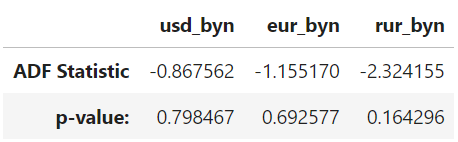
\includegraphics[scale=1.3]{images/tab_1}
		\label{fig:tab1}
	\end{figure}
	
	Как мы можем видеть, для каждого значения валюты у нас принимается гипотеза о том, что временной ряд нестационарный. Проведем преобразования для удаления тренда и сезонности. Например, для курса доллара к белорусскому рублю после проведенных преобразований мы будем иметь следующую зависимость значения курса доллара от даты (Рис. 1):
	
	\begin{figure}[h!]
		\centering
		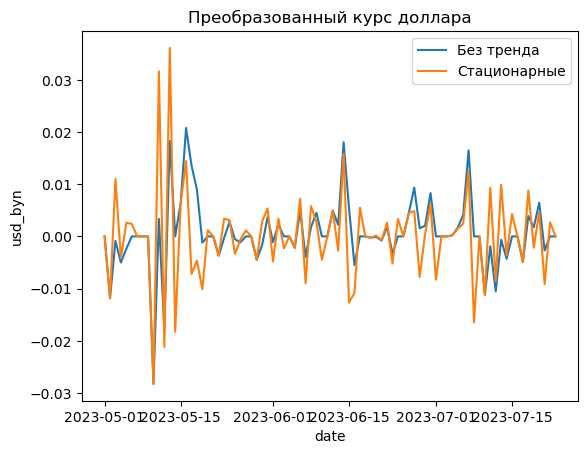
\includegraphics[scale=1.0]{images/pic_01}
		\caption[Рис. 1]{Преобразованный курс доллара}
		\label{fig:pic01}
	\end{figure}
	
	Для проверки снова выдвигаем гипотезу о том, что временные ряды курса валют нестационарные. Используем тест Дики-Фуллера на преобразованных временных рядах и получим следующее (Таблица 2):
	
	\begin{figure}[h!]
		\centering
		\label{fig:tab2}
		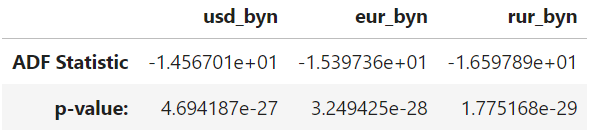
\includegraphics[scale=1.3]{images/tab_2}
	\end{figure}
	
	Таким образом, сейчас мы модем отклонить гипотезу о том, что наши преобразованные временные ряды являются нестационарными.
	
	Нам известно, что курсы валют тесно связаны между собой. Действительно, если составить их корреляционную матрицу (Рис. 2), то можно пронаблюдать крайне высокую статистически значимую корреляцию курсов валют друг с другом.
	
	\begin{figure}[tph!]
		\centering
		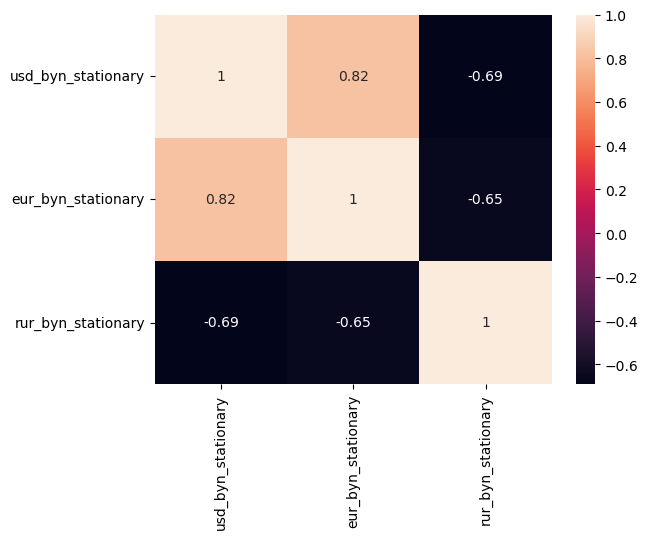
\includegraphics[scale=0.8]{images/pic_02}
		\caption[Рис. 2]{Корреляционная матрица стационарных курсов валют}
		\label{fig:pic02}
	\end{figure}
	
	Это позволяет нам принять решение о том, что в качестве объясняющей переменной мы можем использовать только один из этих курсов с целью улучшения прогнозов модели и избежания мультиколлинеарности признаков.
	
	\subsubsection{Предобработка объясняемых переменных}
	
	Мы будем рассматривать две переменные, которые будем прогнозировать с помощью временных рядов курсов валют --- это показатель ИПЦ месячной частоты и показатель ИПЦ квартальной частоты.
	
	Построим график зависимости ИПЦ от даты (Рис. 3).
	\begin{figure}[bph!]
		\centering
		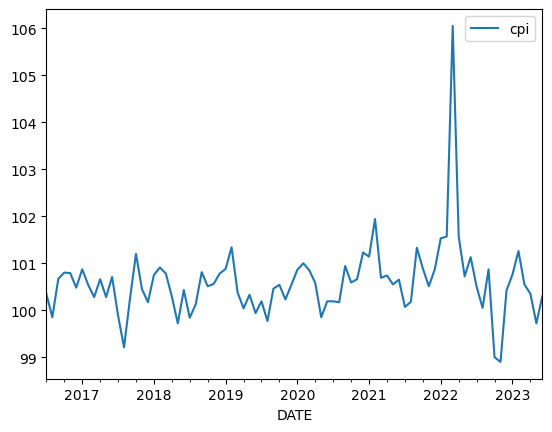
\includegraphics[scale=0.8]{images/pic_03}
		\caption[Рис. 3]{График зависимости ИПЦ месячной частоты от даты}
		\label{fig:pic03}
	\end{figure}
	
	Для того, чтобы использовать этот временной ряд в модели, нам необходимо провести сезонную корректировку этого временного ряда. Сезонная корректировка позволяет устранить сезонные колебания и выделить трендовую и остаточную составляющие временного ряда. Для этого мы сделаем сезонную декомпозицию данного временного ряда. С помощью декомпозиции мы смогли выделить такие компоненты временного ряда как тренд, сезонность и остатки. Вычитая из исходного временного ряда компоненту сезонности, получим сезонно скорректированный временной ряд ИПЦ (Рис. 4).
	\begin{figure}[tph!]
		\centering
		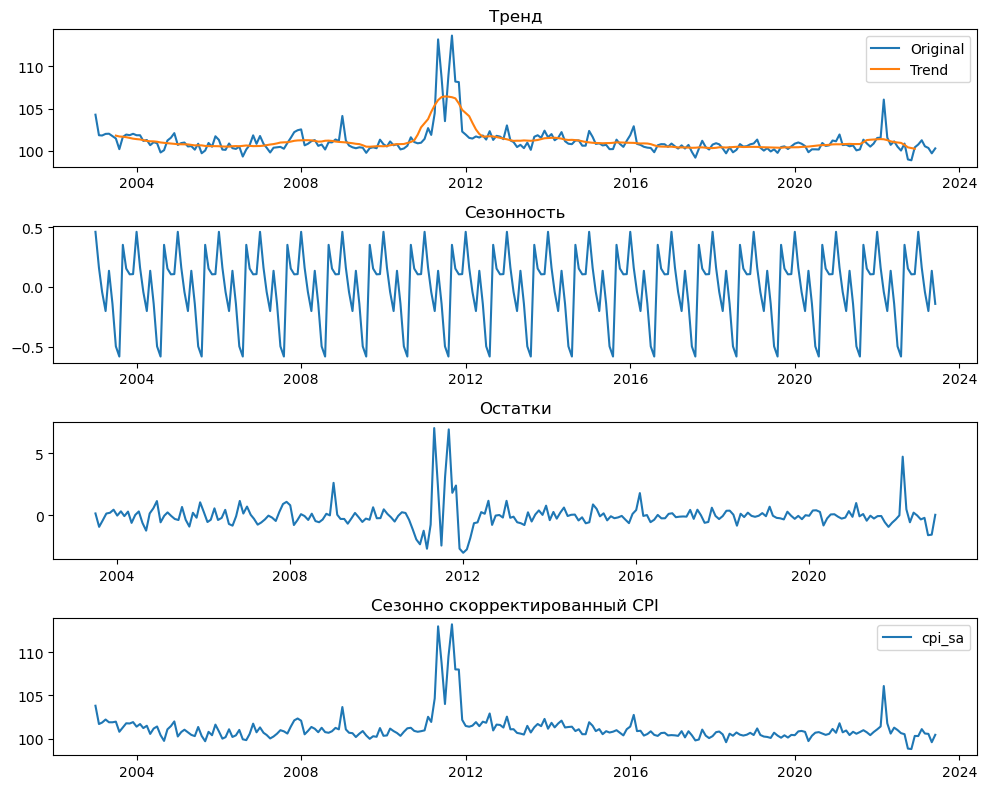
\includegraphics[scale=0.5]{images/pic_04}
		\caption[Рис. 4]{Сезонная декомпозиция временного ряда ИПЦ месячной частоты}
		\label{fig:pic04}
	\end{figure}
	
	На графике сезонности явно прослеживается повторение каждый год.
	Построим график темпов роста сезонно скорректированного ИПЦ месячной частоты (Рис. 5).
	
	\begin{figure}[bph!]
		\centering
		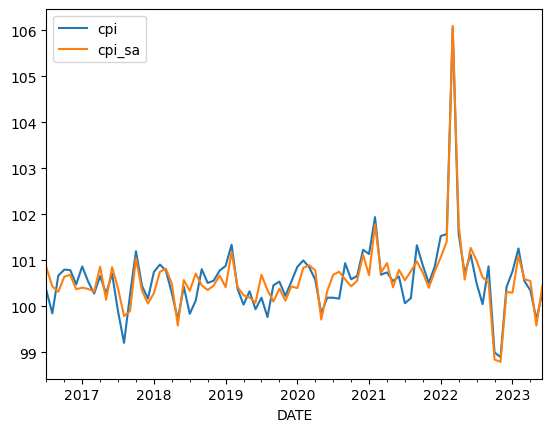
\includegraphics[scale=0.8]{images/pic_05}
		\caption[Рис. 5]{График темпов роста сезонно скорректированного ИПЦ месячной частоты}
		\label{fig:pic05}
	\end{figure}
	
	Аналогичным образом поступим с временным рядом ИПЦ квартальной частоты: сделаем сезонную декомпозицию и построим график темпов роста сезонно скорректированного ИПЦ квартальной частоты (Рис.6, Рис. 7).
	
	\begin{figure}[tph!]
		\centering
		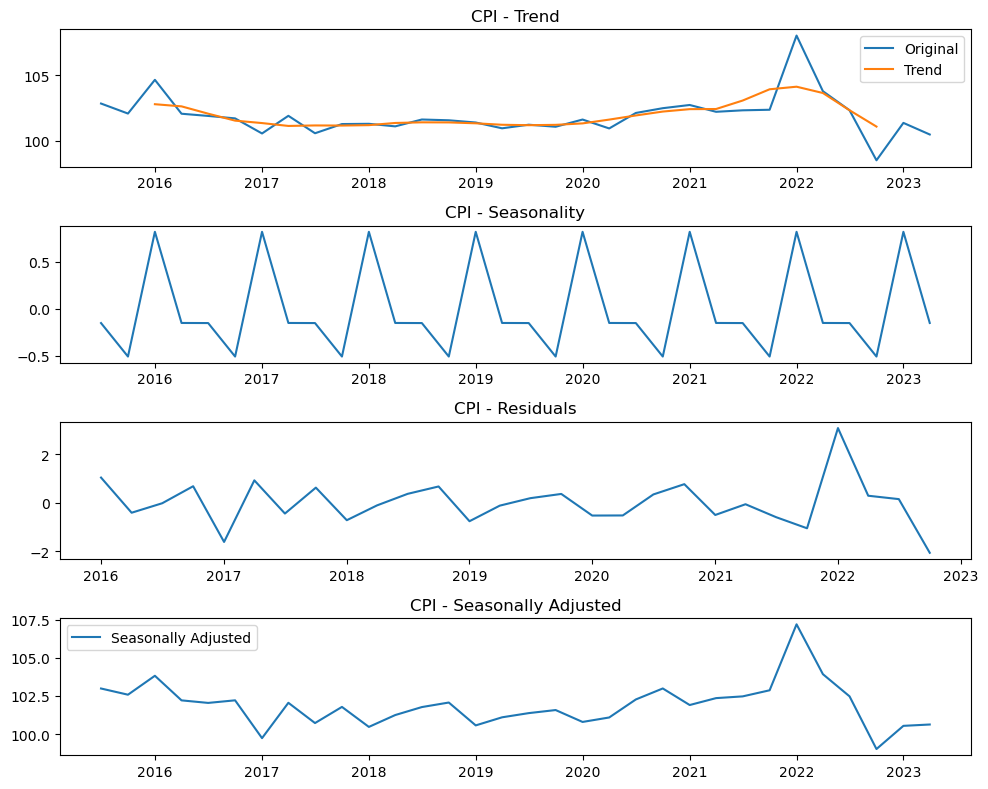
\includegraphics[scale=0.6]{images/pic_06}
		\caption[Рис. 6]{Сезонная декомпозиция временного ряда ИПЦ квартальной частоты}
		\label{fig:pic06}
	\end{figure}
	
	\begin{figure}[bph!]
		\centering
		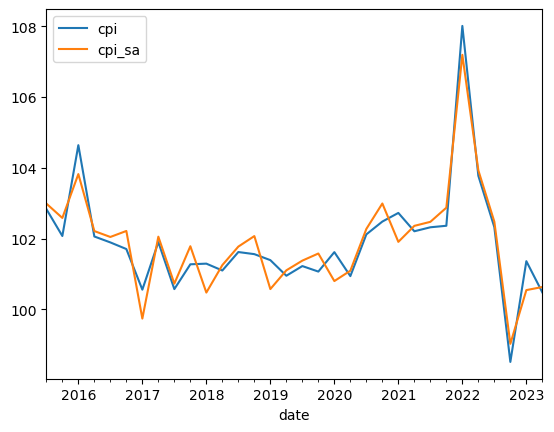
\includegraphics[scale=0.8]{images/pic_07}
		\caption[Рис. 7]{График темпов роста сезонно скорректированного ИПЦ квартальной частоты}
		\label{fig:pic07}
	\end{figure}
	
	\subsection{Прогнозирование месячного показателя ИПЦ по дневному курсу доллара}
	
	Рассмотрение проведем для базовой модели MIDAS регрессии, введенной в пункте 3.3. В качестве примера мы возьмем библиотеку для Python под названием 'midas\_pro', в которой уже реализована базовая модель MIDAS, поддерживающая экспоненциальные лаги Алмона (формула (3.5)) и бета лаги (формула (3.6)).
	
	В качестве объясняющей переменной возьмем курс доллара по отношению к белорусскому рублю (далее курс доллара). Причем возьмем данные о курсе начиная от деноминации от 1 июля 2016-го года.
	
	Мы будем обучать модель на данных с 1 июля 2016-го года до 1 июля 2021-го года, а тестировать --- с 1 августа 2021-го года до 1 июня 2023-го года. В качестве оценки точности модели будем использовать RMSE-оценку и MAE-оценку.
	
	Для применения модели MIDAS нам нужно смешать наши частоты и указать число лагов. Как мы замечали ранее в главе 3 основными гиперпараметрами нашей модели является указание того, какие лаговые многочлены мы будем использовать, и числа лагов этих многочленов. 
	
	\subsubsection{Прогнозирование с использованием лагов Алмона}
	Рассмотрим экспоненциальные многочлены Алмона, тогда наша модель задается формулой $$y_t = \lambda + \sum_{j=0}^{K_1}\beta_j  \dfrac{e^{\Theta_1 j + \ldots \Theta_n j^n}}{\sum_{s=0}^{K_2}e^{\Theta_1 s + \ldots \Theta_n s^n}} L^{j/m} x_t^{(m)} + \epsilon_t^{(m)}.\eqno (4.1)$$
	У нас остались не заданными такие гиперпараметры как $K_1$ и $K_2$ --- количество лагов. Далее мы будем менять число лагов и смотреть на те результаты, которые будет выдавать наша модель. 
	
	Таким образом, листинг программы будет следующий:
	\begin{python}
		# mixing the frequencies
		y, yl, x, yf, ylf, xf = mix_freq(cpi.cpi, stat_rates.usd_byn, K_1, K_2, 2,
		start_date=datetime.datetime(2016,7,1),
		end_date=datetime.datetime(2021,7,1))
		
		# training the model
		model = estimate(y, yl, x, poly='expalmon')
		
		# print values of the coefficients
		print(model.x)
		
		# forecasting gdp
		fc = forecast(xf, ylf, model, poly='expalmon')
		
		# print RMSE 
		print(rmse(forecast_df.yfh, cpi.cpi))\end{python}
		\begin{enumerate}
			\item Пусть $K_1 = 1$, $K_2 = 2$. Тогда получаем следующий результат:
			\begin{itemize}
				\item оценки коэффициентов:
				\begin{figure}[h!]
					\centering
					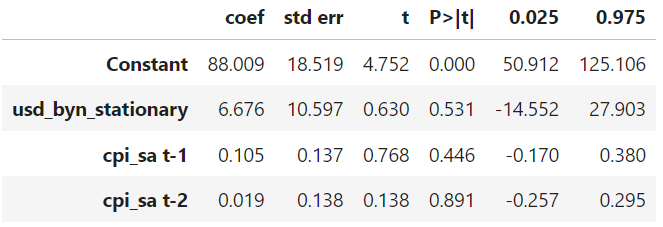
\includegraphics[scale=1.1]{images/tab_3}
					\label{fig:tab3}
				\end{figure}
				
				\item RMSE = 0.36477063424733225
				\item MAE = 0.27117414944638885
				\item график реальной и предсказанной зависимостей (Рис. 8)
				\begin{figure}[h!]
					\centering
					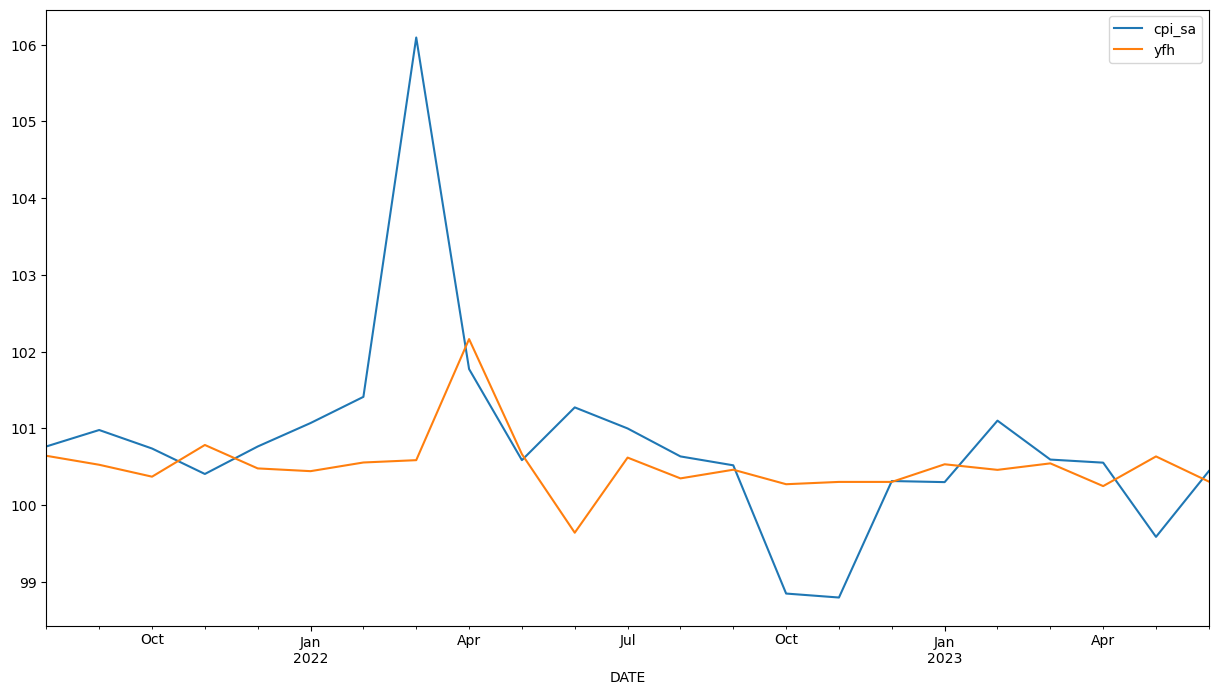
\includegraphics[scale=0.4]{images/pic_08}
					\caption[Рис. 8]{График реального и предсказанного ИПЦ при $K_1 = 1$, $K_2 = 2$.}
					\label{fig:pic08}
				\end{figure}
				
			\end{itemize}
			
			\item Пусть $K_1 = 2$, $K_2 = 4$. Тогда получаем следующий результат:
			\begin{itemize}
				\item оценки коэффициентов \begin{figure}[h!]
					\centering
					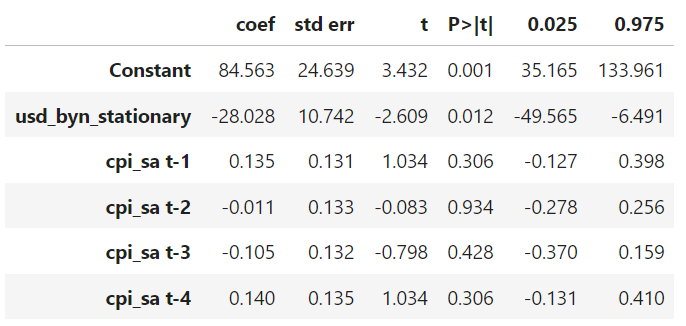
\includegraphics[scale=1.1]{images/tab_5}
					\label{fig:tab5}
				\end{figure}
				
				\item RMSE = 1.3601253119396524;
				\item MAE = 0.7460288917755717;
				\item график реальной и предсказанной зависимостей (Рис. 9)
				\begin{figure}[h!]
					\centering
					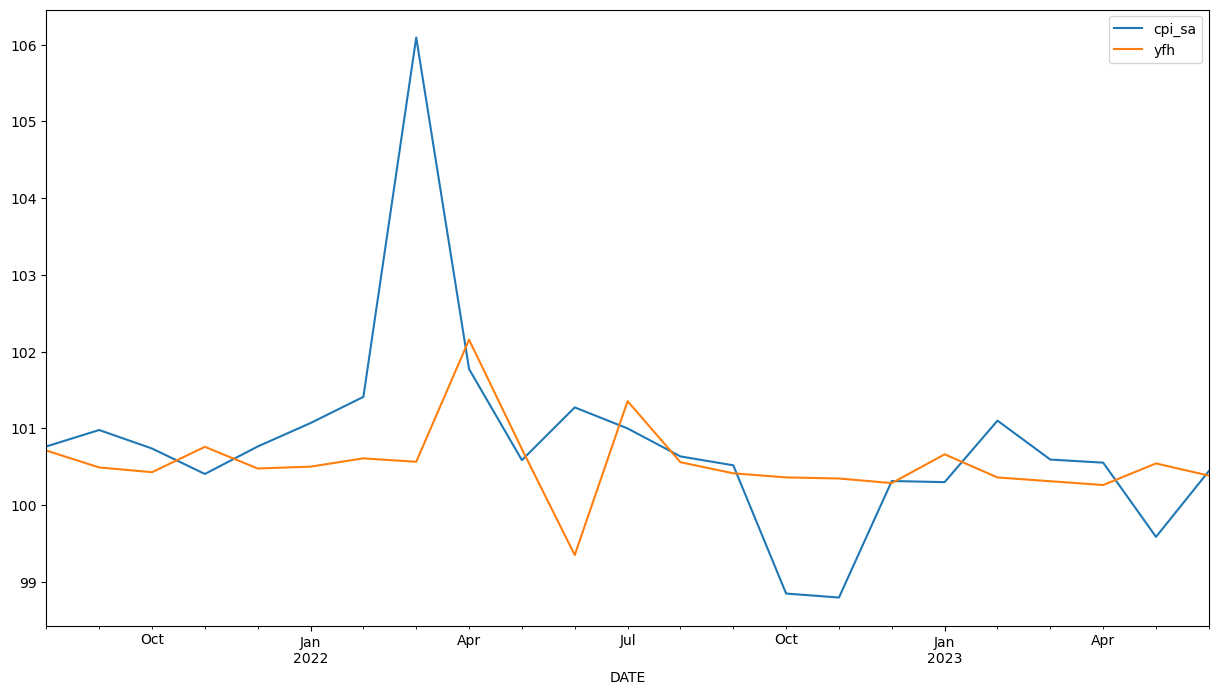
\includegraphics[scale=0.4]{images/pic_09}
					\caption[Рис. 9]{График реального и предсказанного ИПЦ при $K_1 = 2$, $K_2 =4$.}
					\label{fig:pic09}
				\end{figure}
				
			\end{itemize}
			
			Попробуем уменьшить период прогнозирования до трех месяцев.
			
			\item Пусть $K_1 = 4$, $K_2 = 6$. Тогда получаем следующий результат:
			\begin{itemize}
				\item оценки коэффициентов:
				\begin{figure}[h!]
					\centering
					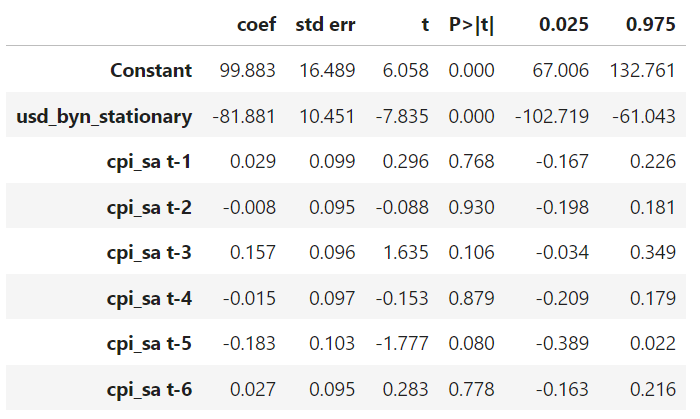
\includegraphics[scale=1.1]{images/tab_6}
					\label{fig:tab6}
				\end{figure}
				
				\item RMSE = 0.6569496548605925;
				\item MAE = 0.5253274032652087;
				\item график реальной и предсказанной зависимостей (Рис. 10)
				\begin{figure}[h!]
					\centering
					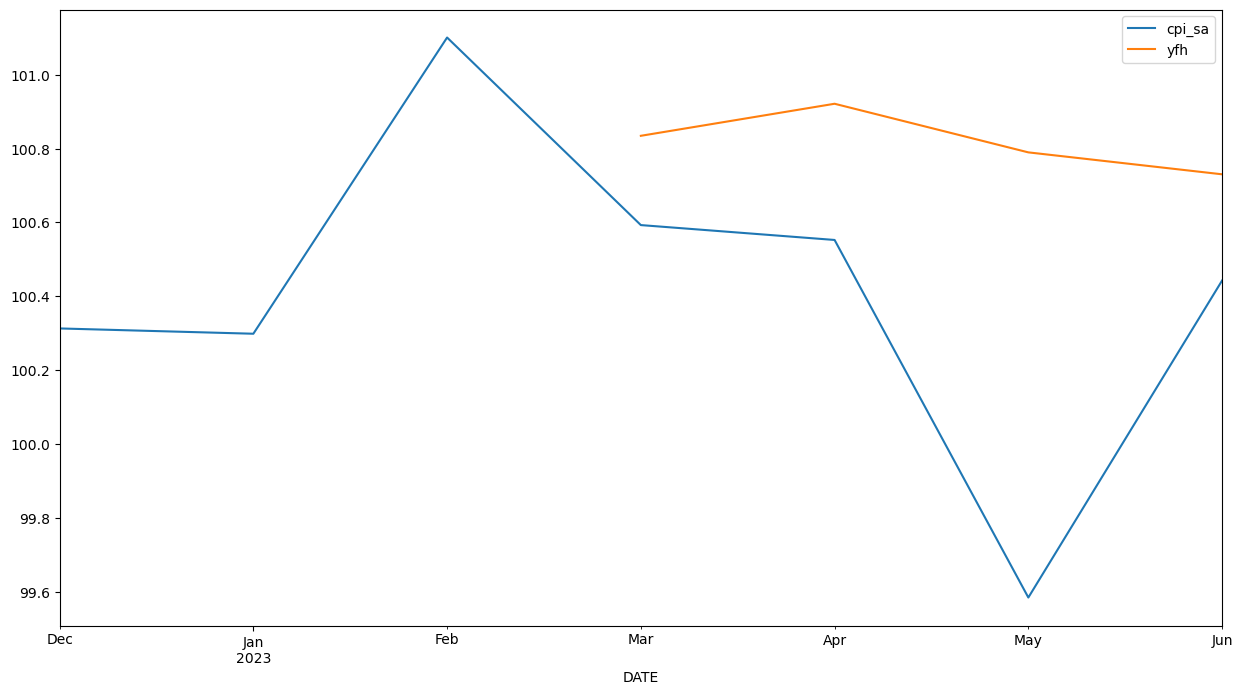
\includegraphics[scale=0.4]{images/pic_10}
					\caption[Рис. 10]{График реального и предсказанного ИПЦ при $K_1 = 4$, $K_2 = 6$.}
					\label{fig:pic10}
				\end{figure}
				
			
		\end{itemize}
		
			\item Пусть $K_1 = 3$, $K_2 = 1$. Тогда получаем следующий результат:
			\begin{itemize}
				\item оценки коэффициентов:
				\begin{figure}[h!]
					\centering
					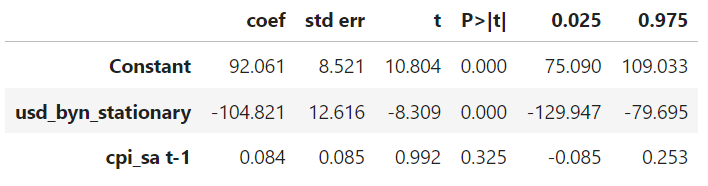
\includegraphics[scale=1.1]{images/tab_7}
					\label{fig:tab7}
				\end{figure}
				
				\item RMSE = 0.5340301272485823;
				\item MAE = 0.3625072971582952
				\item график реальной и предсказанной зависимостей (Рис. 11)
				\begin{figure}[tph!]
					\centering
					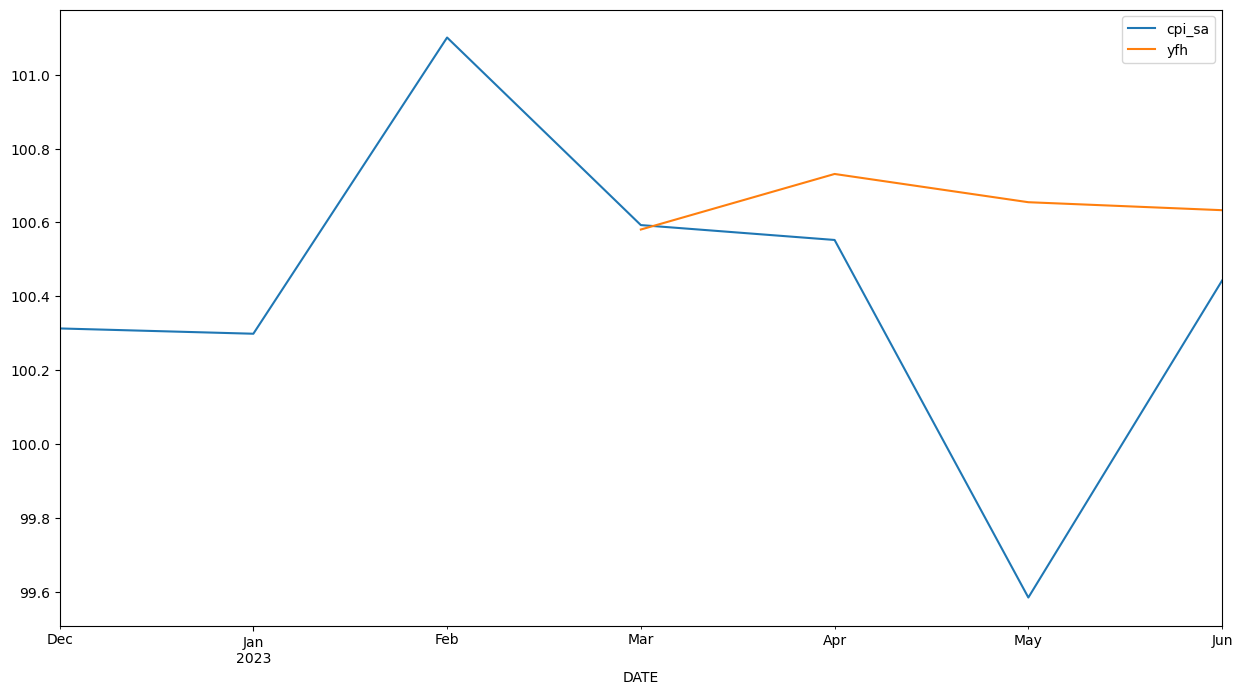
\includegraphics[scale=0.4]{images/pic_11}
					\caption[Рис. 11]{График реального и предсказанного ИПЦ при $K_1 = 3$, $K_2 = 1$.}
					\label{fig:pic11}
				\end{figure}
			\end{itemize}
		\end{enumerate}
		\subsubsection{Прогнозирование с использованием бета лагов}
		Рассмотрим лаговые бета многочлены, тогда наша модель задается формулой $$y_t = \lambda + \sum_{j=0}^{K_1}\dfrac{f(\frac j K, \Theta_1;\Theta_2)}{\sum_{s=0}^{K_2}f(\frac s K, \Theta_1;\Theta_2)} L^{j/m} x_t^{(m)} + \epsilon_t^{(m)}.\eqno (4.2)$$
		Мы не будем приводить такое количество примеров, как для предыдущего случая, так как кардинальных отличий мы не увидим. Приведем один пример. Возьмем $K_1 = 1$ и $K_2 = 3$. Тогда показатели будут следующие:\begin{itemize}
			\item оценки коэффициентов:
			$$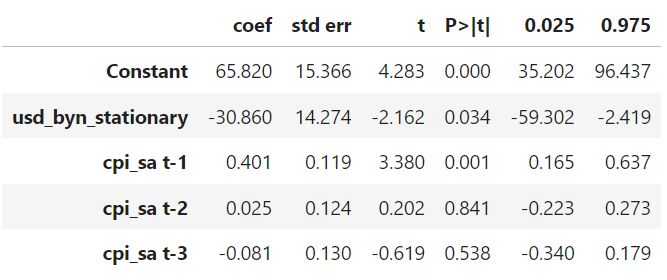
\includegraphics[scale=1.1]{images/tab_8}$$
			
			
			\item RMSE = 0.5340301272485823;
			\item MAE = 0.3625072971582952
			\item график реальной и предсказанной зависимостей (Рис. 12)
			\begin{figure}[bh!]
				\centering
				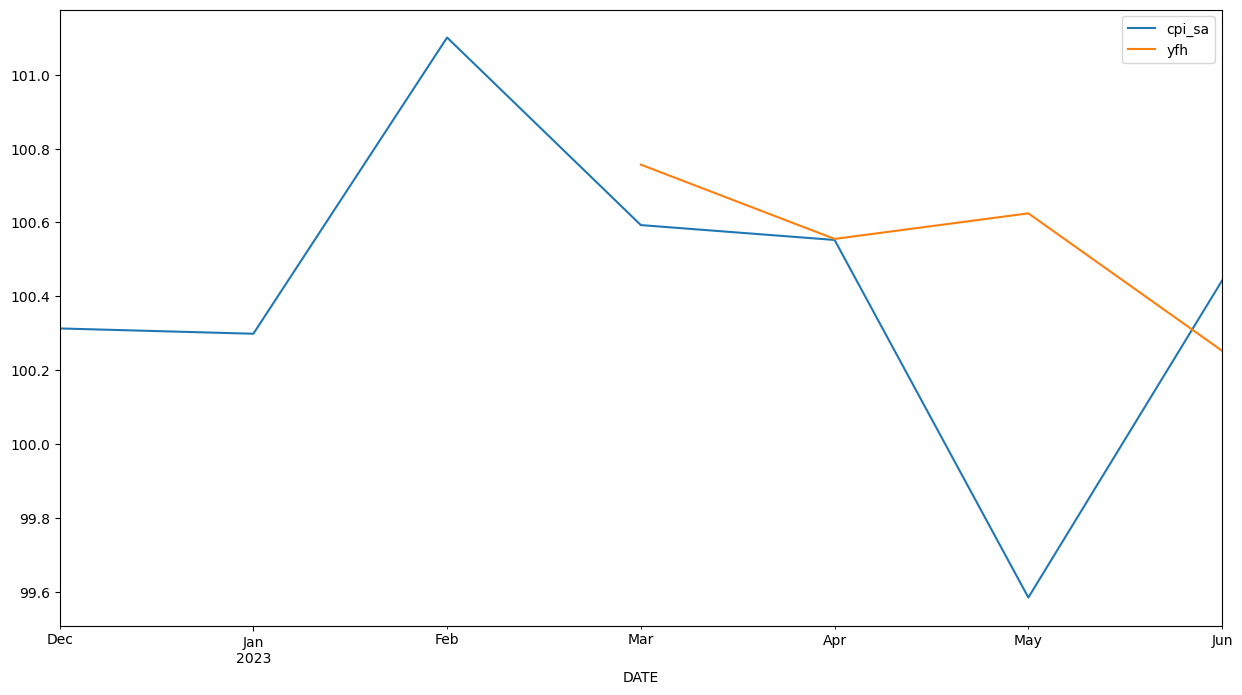
\includegraphics[scale=0.4]{images/pic_12}
				\caption[Рис. 12]{График реального и предсказанного ИПЦ при $K_1 = 1$, $K_2 = 3$.}
				\label{fig:pic12}
			\end{figure}
		\end{itemize}
		
		
		Таким образом, мы можем сделать вывод, что на результаты прогнозирования не так сильно влияет способ задания лагового многочлена, как степень этого многочлена. При слишком большой степени лагового многочлена прогноз начинает ухудшаться, поэтому лучше перебирать среди достаточно низких степеней. На практике выбор степени многочлена будет зависеть непосредственно от поставленной задачи и допустимой ошибки прогнозирования.
		
		\subsection{Прогнозирование квартального показателя ИПЦ по дневному курсу валют}
		Пусть теперь объясняющей переменной будет курс российского рубля по отношению к белорусскому рублю (далее курс российского рубля), а объясняемая переменная, то есть ИПЦ, будет на квартальной частоте.
		
		В отличие от значений предыдущего случая, мы имеем в 3 раза меньше значений ИПЦ. Поэтому теперь мы будем обучать модель на данных с 1 июля 2016-го года до 1 июля 2022-го года, а тестировать --- с 1 августа 2022-го года до 1 июня 2023-го года. То есть мы расширили диапазон значений для обучения и сузили для тестирования. В качестве оценки точности модели мы также будем использовать RMSE-оценку и MAE-оценку.
		
		Все обозначения возьмем из пункта 4.1.1 и снова будем настраивать параметры $K_1$ и $K_2$ --- степени лаговых многочленов.	
		\begin{enumerate}
			\item Пусть $K_1 = 1$, $K_2 = 2$. Тогда
			\begin{itemize}
				\item оценки коэффициентов:
				\begin{figure}[h!]
					\centering
					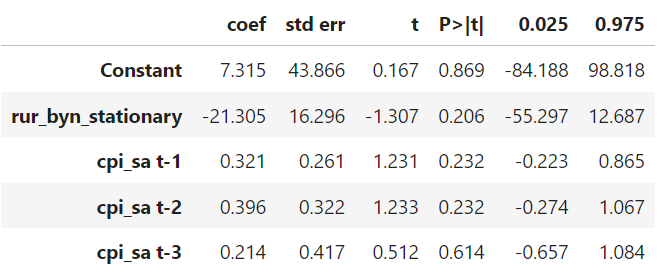
\includegraphics[scale=1.1]{images/tab_9}
					\label{fig:tab9}
				\end{figure}
				
				\item RMSE = 0.5449317099704336;
				\item MAE = 0.5086008381834546;
				
				\item график реальной и предсказанной зависимостей на обучаемых данных  (Рис. 13); 
				\begin{figure}[h!]
					\centering
					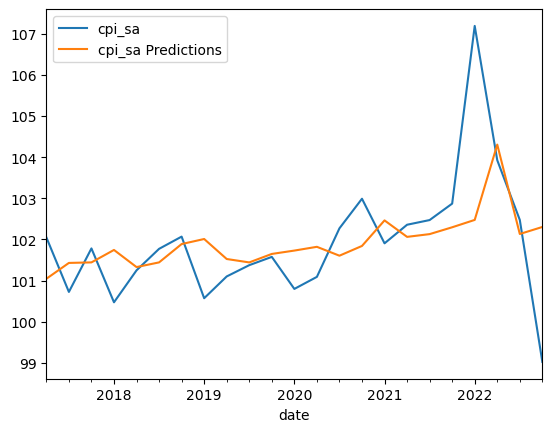
\includegraphics[scale=0.8]{images/pic_13}
					\caption[Рис. 13]{График реального и предсказанного ИПЦ на обучаемых данных при $K_1 = 1$, $K_2 = 2$.}
					\label{fig:pic13}
				\end{figure}
				
				\item график реальной и предсказанной зависимостей на тренировочных данных  (Рис. 14). 
				\begin{figure}[h!]
					\centering
					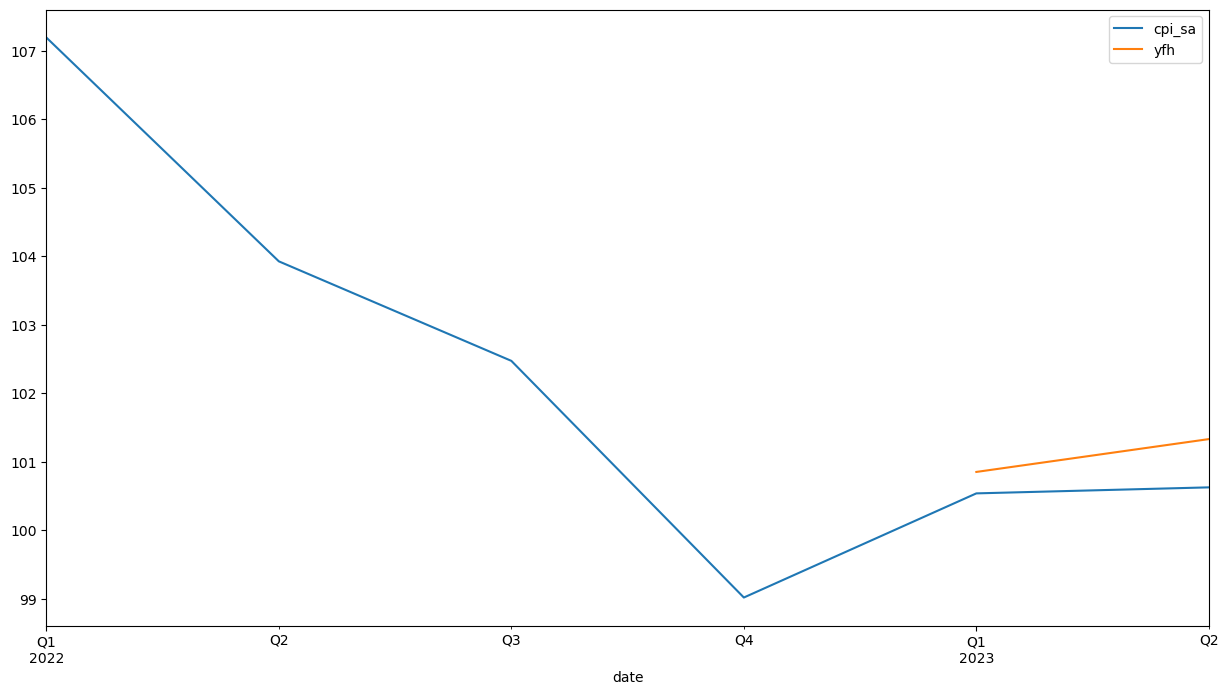
\includegraphics[scale=0.4]{images/pic_14}
					\caption[Рис. 14]{График реального и предсказанного ИПЦ на тренировочных данных при $K_1 = 1$, $K_2 = 2$.}
					\label{fig:pic14}
				\end{figure}
				
			\end{itemize}
			
			\item Пусть $K_1 = 3$, $K_2 = 4$. Тогда
			\begin{itemize}
			\item оценки коэффициентов:
				$$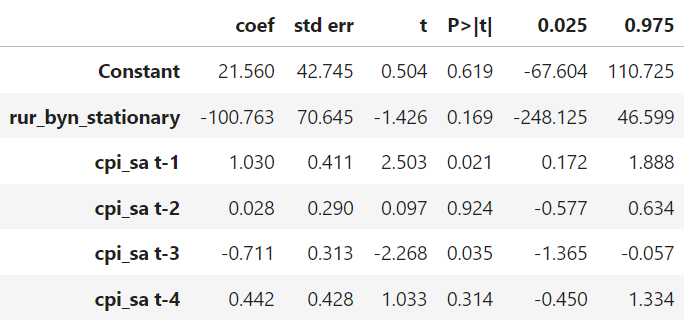
\includegraphics[scale=1.1]{images/tab_10}$$
			
			\item RMSE = 0.22628994850193043;
			\item MAE = 0.16391451978260818;
			
			\item график реальной и предсказанной зависимостей на обучаемых данных  (Рис. 13); 
				\begin{figure}[h!]
					\centering
					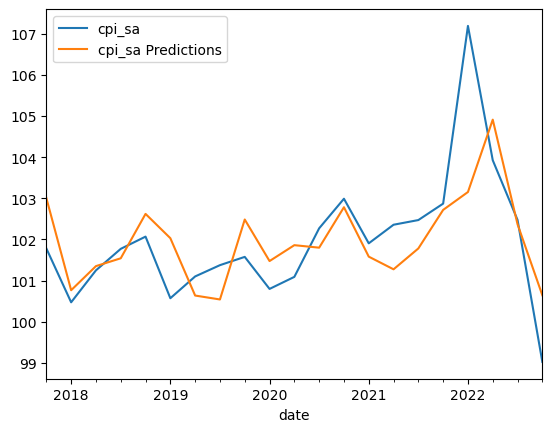
\includegraphics[scale=0.75]{images/pic_15}
					\caption[Рис. 15]{График реального и предсказанного ИПЦ на обучаемых данных при $K_1 = 3$, $K_2 = 4$.}
					\label{fig:pic15}
				\end{figure}
			
			\item график реальной и предсказанной зависимостей на тренировочных данных  (Рис. 16). 
				\begin{figure}[h!]
					\centering
					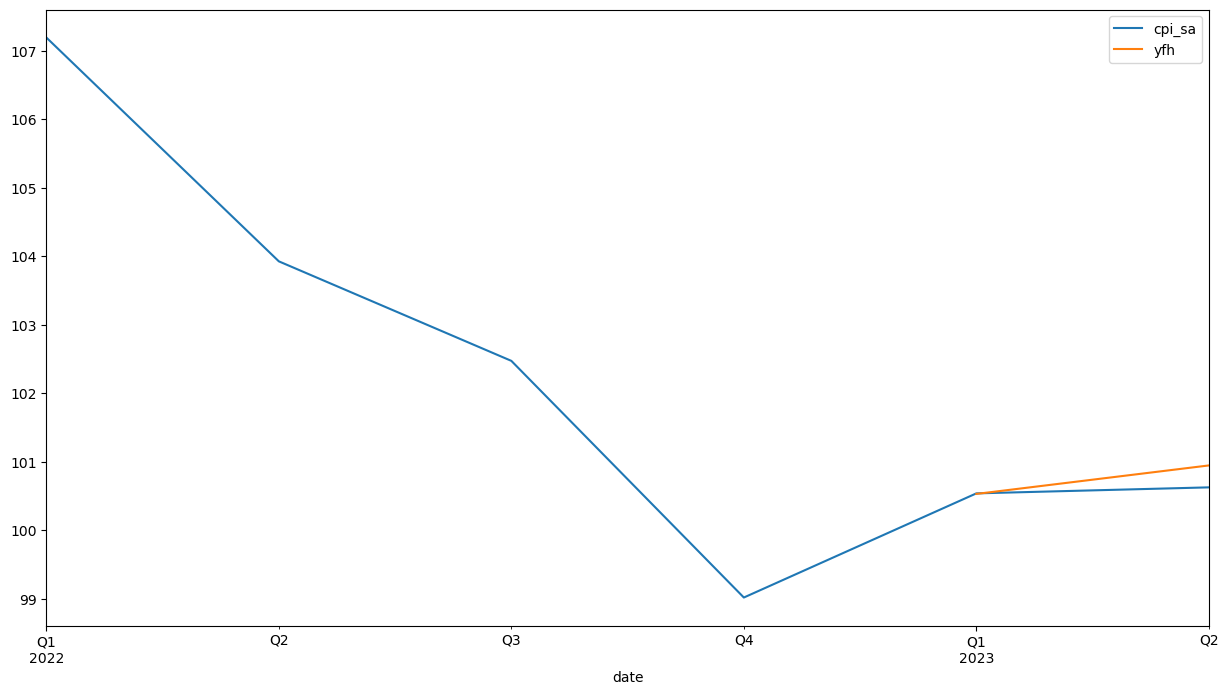
\includegraphics[scale=0.35]{images/pic_16}
					\caption[Рис. 16]{График реального и предсказанного ИПЦ на тренировочных данных при $K_1 = 3$, $K_2 = 4$.}
					\label{fig:pic16}
				\end{figure}
			
			\end{itemize}
		\end{enumerate}
			
			Лучший прогноз наша модель дала при значениях параметров $(3,4)$. А при попытке усложнить модель прогноз становится лишь хуже. 
			
			Наименьшее значение ошибки мы можем получить, взяв в качестве предсказываемого периода лишь один квартал, а все остальные используя для обучения. Если мы расширим период прогнозирования, то ошибки будут еще выше.
	 \newpage
	\section{ЗАКЛЮЧЕНИЕ}
	В данном курсовом проекте мы рассмотрели такую задачу, как предсказывание временных рядом по данными разной частоты, и основные модели, решающие эту задачу. Мы также провели практические исследования модели MIDAS регрессии, которая является одной из основных моделей, решающих поставленную задачу.
	
	На сегодняшний день задача предсказания временных рядов по данным разной частоты остается все еще актуальной, так как мы на практическом примере убедились, что с помощью моделей, способных решать подобную задачу, мы можем прогнозировать значения такого важного макроэкономического показателя как ИПЦ.
	
	Нами были рассмотрены много моделей, работающих с данными разной частоты. Подытоживая, мы можем выделить три основных типа моделей (в зависимости от используемых этими моделями подходов):
	\begin{itemize}
		\item модели MIDAS регрессии;
		\item модели векторной авторегрессии;
		\item динамические факторные модели.
	\end{itemize}
	Все эти модели хорошо себя показывают в прогнозировании временных рядов со смешанными частотами. Выбор модели целиком зависит от поставленной задачи и проведенных исследований. Целесообразно для реальной задачи прогнозирования каких-либо показателей использовать все предложенные модели, чтобы выявить лучший прогноз. Так как для каждой задачи какая-то конкретная модель может показать себя лучше остальных. Проблемой может выступать лишь то, что эти модели реализованы в относительно небольшом числе пакетов, что может затруднять процесс исследований.
	
	Нами также были рассмотрены основные критерии, применяемые для оценки качества прогнозов моделей. Но на практике выбор критерия также зависит непосредственно от данных. Как и с моделями, целесообразнее будет использовать сразу несколько различных оценок качества прогнозов и стараться минимизировать, если и не все, то большинство этих оценок.
	
	В 4 главе нами были проведены практические исследования с использованием модели MIDAS регрессии для предсказания реальных временных рядов. Исходя из проведенных исследований, можем заключить, что, используя модель MIDAS регрессии, мы можем с некоторой небольшой ошибкой предсказывать значения месячной переменной по значениям дневной переменной. Однако на результаты прогноза также могут влиять и физические факторы, например то, насколько сильная взаимосвязь между рассматриваемыми переменными.
	
	Проведенные нами исследования позволяют сделать и более глобальные выводы. Например, мы убедились, что существует тесная взаимосвязь между темпами роста показателя ИПЦ в квартальном выражении с ежедневными темпами роста обменного курса валют.
	\newpage
	\section{СПИСОК ИСТОЧНИКОВ}
	\begin{enumerate}
		\item Foroni, C. A survey of econometric methods for mixed frequency data / C. Foroni, M. Marcellino // Working Paper 2013/06, Norges Bank.
		\item Ghysels, E., Santa-Clara P., Valkanov R. 2002. The MIDAS touch: Mixed data sampling regression models, Working paper, UNC and UCLA.
		\item Макеева, Н.М., Наукастинг элементов использования ВВП России / Н.М. Макеева, И.П. Станкевич // Статья 2022/10, Экономический журнал ВШЭ.
		\item Foroni, C. Unrestricted Mixed Data Sampling (U-MIDAS): MIDAS Regressions With Unrestricted Lag Polynomials / C. Foroni, M. Marcellino, C. Schumacher // Discussion paper 2015, Deutsche Bundesbank.
		\item Станкевич И.П. Сравнение методов наукастинга макроэкономических индикаторов на примере российского ВВП // Прикладная эконометрика 2020. С. 113–127.
		\item Ghysels, E. Regression models with mixed sampling frequencies /  E. Andreou, A. Kourtellos // Journal of Econometrics 2010.
		\item Soybilgen, B. Nowcasting the New Turkish GDP / B. Soybilgen, E. Yazgan // Economics Bulletin, Volume 38, Issue 2, 
		С. 1083-1089
		\item Ghysels, E. MIDAS Regressions: Further Results and New Directions / E. Ghysels, A. Sinko, R. Valkanov // Working paper.
		\item Kuzin, V. MIDAS vs. Mixed-Frequency VAR:
		Nowcasting GDP in the Euro Area / V. Kuzin,
		M. Marcellino, C. Shumacher // EUI Working Paper.
		\item Харин, Ю. С. Теория вероятностей,
		математическая
		и прикладная статистика / Ю. С. Харин, Н. М. Зуев, Е. Е. Жук // Минск : БГУ, 2011. 
	\end{enumerate}
	\newpage
	\section{ПРИЛОЖЕНИЕ}
	Полный листинг программы из главы 4:
	\begin{python}
		# import libraries
	%matplotlib inline
	import matplotlib.pyplot as plt
	import numpy as np
	import pandas as pd
	import datetime
	import seaborn as sns
	from statsmodels.tsa.stattools import adfuller
	from itertools import product
	from statsmodels.tsa.seasonal import seasonal_decompose
	from sklearn.metrics import mean_squared_error, mean_absolute_error
	
	
	from midas.mix import mix_freq, mix_freq2
	from midas.adl import estimate, forecast, midas_adl, rmse, estimate2,forecast2, midas_adl2
		
		# import ex_rates
		ex_rates = pd.read_csv('ex_rates.csv', parse_dates=['DATE'], dayfirst=True, index_col='DATE', sep=';')['2016-07-01':'2023-06-30']
		ex_rates['usd_byn'] = ex_rates['usd_byn'].str.replace(" ", "").astype(float)
		ex_rates['eur_byn'] = ex_rates['eur_byn'].str.replace(" ", "").astype(float)
		ex_rates.tail()
		
		# ADF test for non stationary ex_rates
		usd = adfuller(ex_rates['usd_byn'])
		rur = adfuller(ex_rates['rur_byn'])
		eur = adfuller(ex_rates['eur_byn'])
		
		DF_test = pd.DataFrame([[usd[0], eur[0], rur[0]], [usd[1], eur[1], rur[1]]], index=["ADF Statistic", "p-value:"], columns=["usd_byn", "eur_byn", "rur_byn"])
		DF_test
		
		# delete trend
		ex_rates['usd_byn_no_trend'] = ex_rates['usd_byn'] - ex_rates['usd_byn'].rolling(window=2).mean()
		
		# delete seasonality
		ex_rates['usd_byn_stationary'] = ex_rates['usd_byn_no_trend'].diff()
		ex_rates.dropna(inplace=True)
		
		# plot usd_byn ex_rate
		plt.plot(ex_rates['usd_byn_no_trend']['2023-05-01':], label='no trend')
		plt.plot(ex_rates['usd_byn_stationary']['2023-05-01':], label='stationary')
		plt.legend()
		plt.xlabel('date')
		plt.ylabel('usd_byn')
		plt.show()
		
	# making eur_byn and rur_byn stationary
	ex_rates['eur_byn_no_trend'] = ex_rates['eur_byn'] - ex_rates['eur_byn'].rolling(window=2).mean()
	ex_rates['eur_byn_stationary'] = ex_rates['eur_byn_no_trend'].diff()
	ex_rates.dropna(inplace=True)
	ex_rates['rur_byn_no_trend'] = ex_rates['rur_byn'] - ex_rates['rur_byn'].rolling(window=2).mean()
	ex_rates['rur_byn_stationary'] = ex_rates['rur_byn_no_trend'].diff()
	ex_rates.dropna(inplace=True)
	
	#ADF test for stationary ex_rates
	usd = adfuller(ex_rates['usd_byn_stationary'])
	rur = adfuller(ex_rates['eur_byn_stationary'])
	eur = adfuller(ex_rates['rur_byn_stationary'])
	
	DF_test = pd.DataFrame([[usd[0], eur[0], rur[0]], [usd[1], eur[1], rur[1]]], index=["ADF Statistic", "p-value:"], columns=["usd_byn", "eur_byn", "rur_byn"])
	DF_test
		
	# create correlation matrix
	sns.heatmap(ex_rates[['usd_byn_stationary', 'eur_byn_stationary', 'rur_byn_stationary']].corr(), annot = True)
	None
	
	#import cpi
	gdp_cpi = pd.read_csv('gdp_cpi_mm.csv', parse_dates=['DATE'], dayfirst=True, index_col='DATE', sep=';')
	gdp_cpi = gdp_cpi.rename(columns={'GDP' : 'gdp', 'CPI' : 'cpi'})
	cpi = gdp_cpi[['cpi']]
	cpi.loc['2016-07-01':].plot()
	None
	
	# season decomposition
	decomposition = seasonal_decompose(cpi.cpi, model='additive', period=12)
	
	# getting trend, seasonality, residuals
	trend = decomposition.trend
	seasonal = decomposition.seasonal
	residuals = decomposition.resid
	
	# plot results
	plt.figure(figsize=(10, 8))
	
	# show trend
	plt.subplot(411)
	plt.plot(cpi.cpi, label='Original')
	plt.plot(trend, label='Trend')
	plt.legend(loc='best')
	plt.title('best')
	
	# show seasonality
	plt.subplot(412)
	plt.plot(seasonal)
	plt.title('seasonality')
	
	# show residuals
	plt.subplot(413)
	plt.plot(residuals)
	plt.title('residuals')
	
	cpi_sa = pd.DataFrame(cpi.cpi - seasonal, columns=['cpi_sa'])
	
	# show cpi seasonaly adjusted
	plt.subplot(414)
	plt.plot(cpi_sa, label='cpi_sa')
	plt.legend(loc='best')
	plt.title('seasonaly adjusted CPI')
	
	plt.tight_layout()
	plt.show()
	
	# plot cpi and cpi_sa
	pd.concat([cpi, cpi_sa], axis=1).loc['2016-07-01':].plot()
	None
		
		# exp almon lags
		# mixing frequencies & estimation
		K_1 = 1
		K_2 = 2
		y, yl, x, yf, ylf, xf = mix_freq(cpi_sa.cpi_sa, ex_rates.usd_byn_stationary, K_1, K_2, 2,
		start_date=datetime.datetime(2016,7,1),
		end_date=datetime.datetime(2021,7,1))
		
		model = estimate(y, yl, x, poly='expalmon')
		print(*model.x)
		#opt params [beta0, beta1, beta2, theta11, theta12, theta21, theta22, lambda]
		
		# forecasting
		fc = forecast(xf, ylf, model, poly='expalmon')
		forecast_df = fc.join(yf)
		forecast_df['residual'] = forecast_df.yfh - forecast_df.cpi_sa
		print('RMSE =', np.sqrt(mean_squared_error(cpi_sa[['cpi_sa']].loc['2021-08-01':'2023-06-01'], forecast_df.yfh)))
		print('MAE =', mean_absolute_error(cpi_sa[['cpi_sa']].loc['2021-08-01':'2023-06-01'], forecast_df.yfh))
		forecast_df.head()
		
		# plot real cpi & forecasted cpi
		df_cpi = pd.concat([cpi_sa['cpi_sa']['2021-08-01':'2023-06-01'], forecast_df['yfh']], axis=1)
		df_cpi[['cpi_sa', 'yfh']].plot(figsize=(15,8), style=['-', '-'])
		None
	\end{python}
\end{document}